\documentclass[10pt,twocolumn,letterpaper]{article}
\usepackage[pagenumbers]{cvpr}
\usepackage{times}
\usepackage{epsfig}
\usepackage{graphicx}
\usepackage{amsmath}
\usepackage{amssymb}
\usepackage{booktabs}
\usepackage{multirow}
\usepackage{array}
\usepackage{xcolor}
\usepackage{colortbl}
\usepackage{algorithm}
\usepackage{algpseudocode}
\usepackage{placeins}
\usepackage{float}
\usepackage{chngcntr}
\usepackage[pagebackref=false,breaklinks=true,colorlinks=true,citecolor=cvprblue,linkcolor=cvprblue,urlcolor=cvprblue]{hyperref}

\definecolor{cvprblue}{rgb}{0.21,0.49,0.74}
\definecolor{prismred}{HTML}{B91C1C}
\definecolor{prismblue}{HTML}{1D4ED8}
\definecolor{prismteal}{HTML}{0F766E}

\newcommand{\method}{PRISM}
\newcommand{\para}[1]{\par\smallskip\noindent\textbf{#1}\quad}
\newcommand{\best}[1]{\textcolor{prismred}{\textbf{#1}}}
\newcommand{\runnerup}[1]{\textcolor{prismblue}{\underline{#1}}}
\newcommand{\sd}[2]{#1{\scriptsize$\pm$#2}}

\newcommand{\rtts}{RTTS}
\newcommand{\fattal}{Fattal}
\newcommand{\rttssub}{RTTS-128}
\newcommand{\dense}{Dense-Haze}


\title{PRISM: Perceptually Feasible Low-Rank Layer Allocation\\via Decoupled Probing for Real-World Image Dehazing}
\author{Anonymous Author(s)}

\begin{document}
\maketitle
\raggedbottom

\begin{abstract}
Adapting a frozen dehazing backbone under unpaired supervision and a strict parameter budget requires deciding where to place low-rank adapters. Relying solely on local crop-level CLIP haze-to-clear (H2C) loss induces a semantic--perceptual mismatch: 16-block bi-level gating drifts across seeds into narrow encoder layers, while unconstrained bottleneck minimization picks shallow-inclusive subsets that over-enhance sky--facade boundaries. We propose PRISM, decoupling discrete layer selection from gradient updates via Conv-EVA initialization, a 5-epoch 16-block warm-up, and gradient-free enumeration over all $\binom{8}{3}=56$ iso-budget bottleneck subsets on the shared snapshot under a whole-image MUSIQ guardrail. PRISM locks $\{6,7,8\}$ (3.03\% parameters) across all three seeds for unmodified H2C fine-tuning and lossless merging. At identical baseline FLOPs, it cuts RTTS ($n=4322$) FADE by 13.0\% over matched-protocol $\{1,7,8\}$ (17.0\% over reported BiLaLoRA), complemented by cross-domain sensitivity ablations against direct MUSIQ maximization.
\par\smallskip\noindent{\normalfont\textbf{Keywords:}\quad Unpaired image dehazing, low-rank adaptation, semantic--perceptual mismatch, decoupled layer selection, lossless reparameterization.}
\end{abstract}

\section{Introduction}
Single-image dehazing aims to invert scene radiance $J(x)$ from an observation $I(x)$ degraded by atmospheric scattering. Under the classical physical scattering model~\cite{dcp2009,fattal2014}, $I(x) = J(x)t(x) + A(1 - t(x))$, where $t(x)=e^{-\beta d(x)}$ denotes medium transmission and $A$ is global atmospheric light. Because synchronized haze-free ground-truth pairs are rarely attainable for dynamic outdoor scenes, restoration backbones trained primarily on synthetic benchmarks---such as MSBDN~\cite{msbdn2020}, DeHamer~\cite{dehamer2022}, and DEA-Net~\cite{dea2024}---suffer pronounced domain shift when deployed on real-world photography: persistent gray veiling often remains in distant regions, alongside tonal distortion and contrast collapse in low-light areas~\cite{reside2019,dad2020,psd2021}. Adapting a frozen backbone toward authentic real-world distributions without paired supervision or added inference cost remains a central challenge.

Toward this goal, BiLaLoRA~\cite{bilalora2026} attaches low-rank adapters (LoRA)~\cite{lora2022} to 16 candidate residual blocks across DEA-Net's encoder and Level-3 bottleneck (4 blocks each in \texttt{down\_level1} and \texttt{down\_level2}, plus 8 blocks $D_1$--$D_8$ in \texttt{level3}) and trains a 5-epoch bi-level search under a CLIP-based~\cite{clip2021} haze-to-clear (H2C) directional loss before retaining top-$b=3$ blocks (3.03\% of backbone parameters when all three lie in \texttt{level3}) for 25-epoch fine-tuning. Yet achieving both strong haze removal and natural whole-image quality under an equal capacity budget exposes two coupled issues (Figure~\ref{fig:motivation}):

\textbf{(1) Unsupervised Semantic--Perceptual Mismatch.} The H2C loss maximizes cosine displacement of $224\times 224$ random image crops toward clear-scene text embeddings. However, local semantic alignment in CLIP feature space is not equivalent to multi-scale perceptual naturalness across full-resolution imagery~\cite{perception2018,musiq2021}. Exhaustively probing all $\binom{8}{3}=56$ three-block bottleneck subsets on a shared fifth-epoch snapshot $\theta_5$ reveals that purely minimizing H2C selects $\{5,6,8\}$, engaging transition block $D_5$. While this configuration aggressively depresses local fog density (FADE), it induces over-sharpening halos and darkened facade soot at sky--building boundaries (see \texttt{BJ\_Bing\_116} in Figure~\ref{fig:motivation}(b)), dropping whole-image MUSIQ below the reference placement $\{1,7,8\}$.

\textbf{(2) Cross-Seed Structural Drift in Bi-Level Gating.} Under BiLaLoRA's unrestricted 16-block search space, continuous bi-level gates diverge across all three seeds (3407/3408/3409) and drift into narrower encoder layers, collapsing trainable capacity from 110,595 down to 82,947 (\texttt{baseline\_dynamic}: $\{L3_{6,7,8}\}$, $\{L3_{1,6,8}\}$, $\{L3_{6,8},D1_4\}$; RTTS-128 FADE std 0.0507) or 55,299 (\texttt{eva\_dynamic}: $\{L3_{6,7,8}\}$, $\{L3_8,D2_{3,4}\}$, $\{L3_8,D1_{3,4}\}$; FADE std 0.1304). Even after restricting top-3 selection to the 8 equal-capacity Level-3 blocks, gate ranking still diverges on seed 3408---yielding $\{6,7,8\}$, $\{2,6,8\}$, and $\{6,7,8\}$ across seeds 3407--3409 (Figure~\ref{fig:motivation}(a))---increasing RTTS-128 FADE std from 0.0053 to 0.0474.

\begin{figure*}[t]
\centering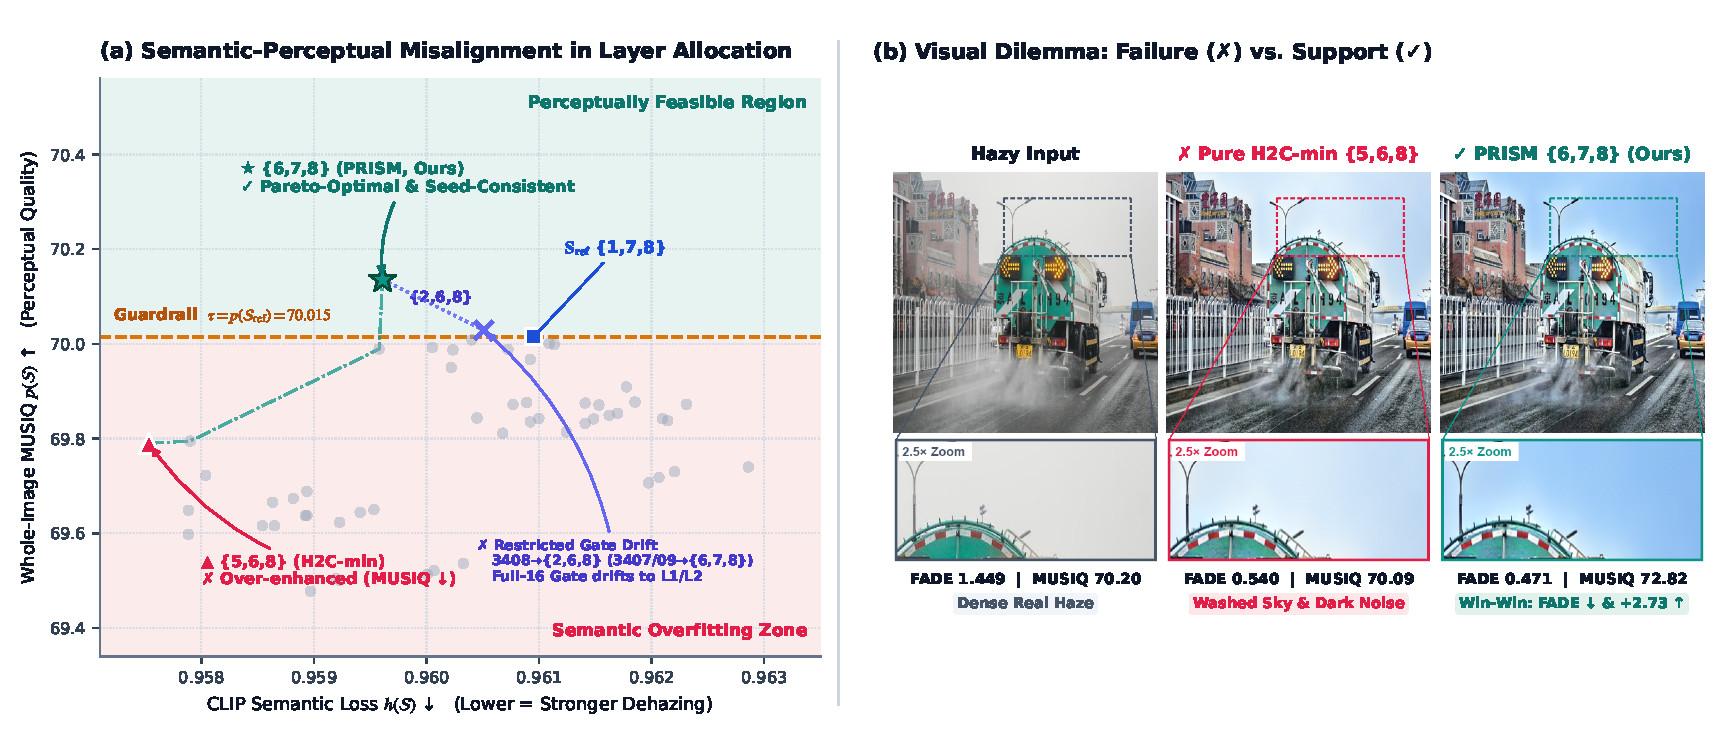
\includegraphics[width=0.96\textwidth]{fig1_motivation.pdf}
\caption{Empirical motivation and semantic--perceptual mismatch. \textbf{(a)} Exhaustive 56-subset Level-3 distribution at shared epoch-5 snapshot $\theta_5$ (seed 3407): unconstrained H2C minimization selects $\{5,6,8\}$ (crimson triangle, $\ell=0.95753$), whose whole-image MUSIQ falls below reference guardrail $\tau=p(\mathcal{S}_{\rm ref})$; restricted gate ranking still drifts to $\{2,6,8\}$ on seed 3408 (while 3407/3409 pick $\{6,7,8\}$ and unrestricted 16-block gating drifts into L1/L2), whereas \method~consistently isolates $\{6,7,8\}$ (teal star). \textbf{(b)} Real-world street scene \texttt{BJ\_Bing\_116} (RTTS-128) with $2.5\times$ crops: relative to $\{5,6,8\}$ sky--facade artifacts (FADE 0.540 / MUSIQ 70.09), \method~delivers deeper dehazing (\best{0.471}) and higher perceptual naturalness (\best{72.82}).}
\label{fig:motivation}
\end{figure*}

To address these limitations, we propose \textbf{\method} (Perceptually Regulated Iso-budget Snapshot Masking), which decouples \textbf{discrete layer allocation from gradient backpropagation}. First, we adapt Explained Variance Adaptation (EVA)~\cite{eva2025} to unfolded 2D convolutional patch space (Conv-EVA), initializing $A_0$ along leading centered covariance eigenvectors of real hazy activations while keeping $B_0=0$ ($\Delta W_0=0$), followed by BiLaLoRA's standard 5-epoch bi-level warm-up over all 16 candidate blocks to produce a shared snapshot $\theta_5$. Second, rather than trusting continuous gate rankings---or backpropagating non-local perceptual scores where they induce conservative under-dehazing shortcuts---we restrict discrete probing to the 8 equal-capacity Level-3 blocks ($\binom{8}{3}=56$ subsets) at $\theta_5$, applying the reference placement's whole-image MUSIQ as guardrail $\tau$ to select the minimum-H2C feasible subset $\{6,7,8\}$. Phase-2 fine-tuning trains only the 3 selected blocks (3.03\% parameters) for 25 epochs under unmodified H2C before lossless linear merging back into the frozen backbone.

Our contributions are summarized as follows:
\begin{enumerate}\setlength{\itemsep}{1pt}\setlength{\parskip}{0pt}
\item \textbf{Quantifying Semantic--Perceptual Mismatch in Unpaired Dehazing}: We map the 56-subset Level-3 decision landscape and per-block marginal sensitivity across $D_1$--$D_8$ on a calibrated epoch-5 snapshot, pinpointing how $D_5$ trades global perceptual quality for local CLIP alignment.
\item \textbf{Decoupled Quality-Guided Probing (\method)}: Combining Conv-EVA initialization with gradient-free, whole-image quality-guided iso-budget probing consistently selects $\{6,7,8\}$ across all three seeds without altering the H2C training objective. We also conduct a 1,232-subset cross-domain and 16-block sensitivity study explicitly separating iso-budget constraint, thresholded two-step selection, and direct MUSIQ maximization.
\item \textbf{Controlled Zero-Overhead Adaptation Gains}: After lossless convolutional merging, \method~updates 3.03\% parameters in phase 2 to cut RTTS ($n=4322$) FADE by 13.0\% over matched-protocol Ref.~\(\{1,7,8\}\)+EVA (17.0\% over reported BiLaLoRA) at identical baseline FLOPs, while transparently characterizing perception--distortion trade-offs on Fattal and Dense-Haze.
\end{enumerate}

\section{Related Work}
\para{Unpaired Supervision for Real-World Dehazing.}
Classical physics-based priors such as Dark Channel Prior~\cite{dcp2009} and Color Lines~\cite{fattal2014} estimate transmission and airlight statistically, but break down near bright skies, white architecture, and non-uniform haze. Deep unpaired approaches broadly follow three paradigms: (i) domain-translation and physical disentanglement frameworks such as DAD~\cite{dad2020}, PSD~\cite{psd2021}, D4~\cite{d42022}, and KANet~\cite{kanet2024}; (ii) clear-domain codebook or contrastive priors including RIDCP~\cite{ridcp2023}, ODCR~\cite{odcr2024}, and IPC~\cite{ipc2025}; and (iii) pseudo-label or physics-guided transfer pipelines (CoRUN~\cite{corun2024}, PHATNet~\cite{phatnet2025}) alongside all-in-one restoration backbones (PromptIR~\cite{promptir2023}, DiffUIR~\cite{diffuir2024}, MoCE-IR~\cite{moce2025}, FoundIR~\cite{foundir2025}). Rather than modifying the backbone architecture or crafting intricate composite losses, we keep the frozen DEA-Net topology and original H2C objective intact and resolve structural layer allocation under an equal parameter budget.

\para{Parameter-Efficient Fine-Tuning \& Subspace Initialization.}
LoRA~\cite{lora2022} freezes pretrained weights and trains parallel low-rank matrices to curtail memory footprint and overfitting. Recent work shows that initialization geometry governs early adaptation under tight budgets: PiSSA~\cite{pissa2024} fine-tunes principal singular components of weights, LoRA-GA~\cite{loraga2024} aligns low-rank subspaces with full-gradient directions, CorDA~\cite{corda2024} builds context-oriented decompositions, and EVA~\cite{eva2025} aligns adapter rows to right singular vectors of input activations, maximizing expected initial gradient norms. In restoration, CoA~\cite{coa2025} adapts compressed representations and BiLaLoRA~\cite{bilalora2026} jointly optimizes layer gates and adapter weights via bi-level gradient descent. We extend EVA to unfolded 2D convolutional tensors (Conv-EVA), suppressing cross-layer activation disparity during short warm-up so a single shared snapshot reliably supports discrete selection.

\para{No-Reference IQA \& Guardrail-Constrained Decisions.}
Blind quality metrics quantify complementary facets of dehazing performance: FADE~\cite{fade2015} estimates residual perceptual fog density via natural scene statistics, BIQME~\cite{biqme2018} evaluates contrast, sharpness, and colorfulness, NIQE~\cite{niqe2013} measures local spatial deviation, and MUSIQ~\cite{musiq2021} applies a multi-scale Transformer trained on KonIQ-10k~\cite{koniq2020} human ratings to capture global structural coherence at native aspect ratios. While prior restoration methods (e.g., RankSRGAN~\cite{ranksrgan2019}) directly inject perceptual evaluators into gradient updates, our controlled diagnostics (Section~\ref{sec:exp_diagnostic}) demonstrate that backpropagating non-local perceptual scores encourages under-dehazing shortcuts. Inspired by hardware-constrained neural architecture search~\cite{mnasnet2019}, \method~isolates whole-image MUSIQ strictly as a gradient-free feasibility constraint during discrete snapshot probing.

\section{Method: PRISM}
\subsection{Conv-EVA Subspace Alignment \& 16-Block Warm-Up}
Pretrained DEA-Net~\cite{dea2024} exposes 16 candidate residual blocks in BiLaLoRA's search space: 4 encoder blocks at \texttt{down\_level1} ($c=32$), 4 at \texttt{down\_level2} ($c=64$), and $M=8$ Content-Guided Attention (CGA) hybrid blocks inside its lowest-resolution ($H/4\times W/4$) Level-3 bottleneck ($c=128$), indexed by $\{D_1,\ldots,D_8\}$. Each block adapts two $3\times 3$ convolutions with weights $W\in\mathbb{R}^{c_o\times c_i\times\kappa\times\kappa}$ ($\kappa=3$). Under contiguous unfolding $\mathcal{R}:\mathbb{R}^{c_o\times c_i\times\kappa\times\kappa}\to\mathbb{R}^{(c_o\kappa)\times(c_i\kappa)}$ and its inverse $\mathcal{R}^{-1}$, a rank-$r$ bypass ($r=8$, inner width $d=r\kappa=24$) forms the effective kernel:
\begin{equation}
W'=W+\Delta W,\qquad \Delta W=\gamma g\,\mathcal{R}^{-1}(BA),
\label{eq:lora}
\end{equation}
where $A\in\mathbb{R}^{d\times c_i\kappa}$ and $B\in\mathbb{R}^{c_o\kappa\times d}$ are low-rank factors, $g=\sigma(u_{\rm gate})\in(0,1)$ is a block-level learnable sigmoid gate shared by the block's two adapted convolutions, and $\gamma=\alpha_{\rm LoRA}/r=2$ ($\alpha_{\rm LoRA}=16$). Restricting the phase-2 selection to budget $b=3$ equal-capacity Level-3 blocks ($c_i=c_o=128$) configures $A\in\mathbb{R}^{24\times 384}$ ($9{,}216$ params) and $B\in\mathbb{R}^{384\times 24}$ ($9{,}216$ params) per layer ($18{,}432$ params/layer), totaling $6\times 18{,}432+3=110{,}595$ trainable parameters---3.03\% of frozen DEA-Net (3,653,377 parameters).

Standard Kaiming uniform initialization leaves $A$ unaligned with real-haze convolutional patch activations. Before warm-up, Conv-EVA runs one frozen forward pass over 32 fixed real hazy training images, samples up to 256 spatial patch positions per image ($N=24{,}576$ unfolded rows across 32 images $\times$ 256 positions $\times$ 3 chunks aligned with $\mathcal{R}$), and computes the centered sample covariance matrix $\Sigma$:
\begin{align}
\mu&=\frac{1}{N}\sum_{j=1}^N x_j, \qquad
\Sigma=\frac{1}{N}(X-\mathbf{1}\mu^\top)^\top(X-\mathbf{1}\mu^\top)=V\Lambda V^\top.
\label{eq:cov}
\end{align}
Taking the top-$d$ orthogonal eigenvectors $V_d^\top\in\mathbb{R}^{d\times(c_i\kappa)}$ in descending eigenvalue order and scaling rows via diagonal matrix $D$ matching each original random row's $\ell_2$ norm yields:
\begin{equation}
A_0=DV_d^\top,\qquad B_0=0\implies \Delta W_0=0.
\label{eq:init}
\end{equation}
Eq.~\eqref{eq:init} aligns each adapter's row space with dominant hazy activation directions while guaranteeing zero initial output drift ($\Delta W_0=0$; Appendix~A.1). Offline patch sampling and covariance eigendecomposition take under 1\,s total. We then follow BiLaLoRA's 5-epoch bi-level warm-up across all 16 candidate blocks under the H2C objective (removing the duplicate input normalization bug in the released branch) to obtain the calibrated shared snapshot $\theta_5$ (Figure~\ref{fig:method}).

\begin{figure*}[t]
\centering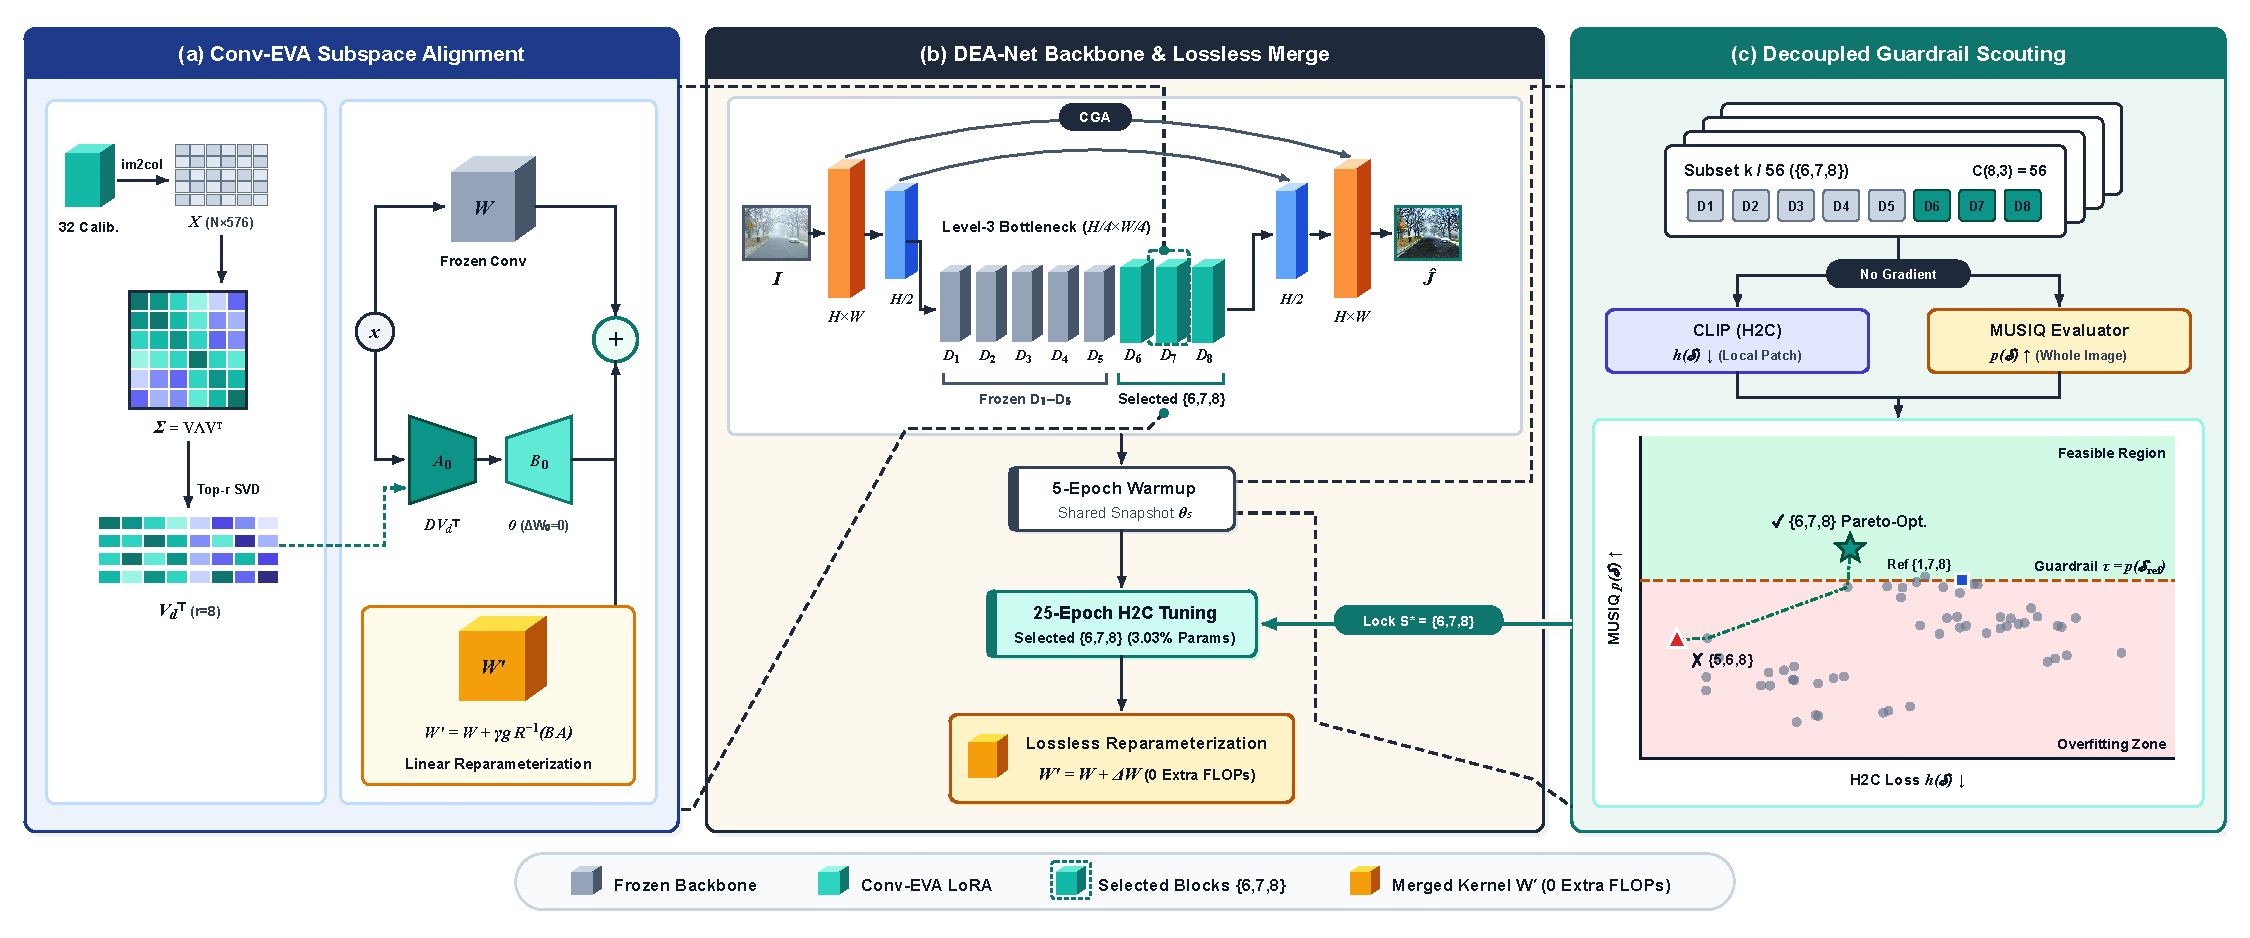
\includegraphics[width=0.96\textwidth]{fig_prism_arch.pdf}
\caption{Overview of \method. \textbf{(a) Conv-EVA Subspace Alignment}: centered covariance $\Sigma=V\Lambda V^\top$ over 32 hazy calibration images initializes zero-perturbation adapters ($A_0=DV_d^\top, B_0=0$); \textbf{(b) DEA-Net Backbone \& Lossless Merging}: after a 5-epoch 16-block bi-level warm-up ($\theta_5$), only selected Level-3 subset $\{6,7,8\}$ (3.03\% params) is fine-tuned for 25 epochs and linearly fused via $W'=W+\Delta W$ at zero FLOP overhead; \textbf{(c) Decoupled Snapshot Probing}: gradient-free enumeration over 56 equal-capacity Level-3 subsets at $\theta_5$ applies guardrail $\tau=p(\mathcal{S}_{\rm ref})$ to reject $\{5,6,8\}$ and select $\{6,7,8\}$.}
\label{fig:method}
\end{figure*}

\subsection{Semantic--Perceptual Mismatch \& Layer Sensitivity}
Let $\mathcal{I}=\{1,\ldots,8\}$ index the 8 equal-capacity Level-3 bottleneck blocks. Under budget $b=3$, the iso-budget candidate space $\Omega_3=\{\mathcal{S}\subset\mathcal{I}:|\mathcal{S}|=3\}$ contains $\binom{8}{3}=56$ discrete subsets. On shared snapshot $\theta_5$, we unmask each candidate $\mathcal{S}$ while silencing the remaining 13 blocks, running gradient-free inference on an isolated 32-image selection split $\mathcal{D}_{\rm sel}$ to evaluate mean crop-level H2C loss $\ell(\mathcal{S})$ and deployment-faithful whole-image MUSIQ $p(\mathcal{S})$ (with 16-multiple bicubic resizing and lossless uint8 projection $\Pi_{\rm deploy}$):
\begin{align}
\ell(\mathcal{S})&=\frac{1}{|\mathcal{D}_{\rm sel}|}\sum_{x\in\mathcal{D}_{\rm sel}}\mathcal{L}_{\rm H2C}\big(f_{\theta_5,\mathcal{S}}(x),x\big), \nonumber\\
p(\mathcal{S})&=\frac{1}{|\mathcal{D}_{\rm sel}|}\sum_{x\in\mathcal{D}_{\rm sel}}\operatorname{MUSIQ}\big(\Pi_{\rm deploy}\big(f_{\theta_5,\mathcal{S}}(x)\big)\big),
\label{eq:probe}
\end{align}
where $\mathcal{L}_{\rm H2C}$ follows BiLaLoRA's CLIP directional cosine distance:
\begin{equation}
\mathcal{L}_{\rm H2C}(y,x)=1-\frac{(\Phi_{\rm img}(y)-\Phi_{\rm img}(x))\cdot(T_{\rm pos}-T_{\rm neg})}{\|\Phi_{\rm img}(y)-\Phi_{\rm img}(x)\|_2\,\|T_{\rm pos}-T_{\rm neg}\|_2}.
\label{eq:h2c}
\end{equation}

Aggregating all 168 subset probes across seeds 3407--3409 reveals each block's marginal inclusion gain $\Delta\mathrm{MUSIQ}$ and semantic gain $-\Delta h$ (Appendix~C, Figure~\ref{fig:sensitivity} and Table~\ref{tab:marginal_blocks}): blocks $D_1$--$D_5$ exhibit uniformly negative average perceptual gain, culminating at $D_5$, which achieves the strongest semantic loss drop ($-\Delta h=+2.06\times 10^{-3}$) alongside the steepest perceptual penalty ($\Delta\mathrm{MUSIQ}=-0.251$). Consequently, unconstrained H2C minimization reliably selects $\{5,6,8\}$, inducing over-enhancement. Conversely, deep blocks $\{D_6,D_7,D_8\}$ all contribute positive perceptual gains ($+0.109/+0.149/+0.130$), with $D_6$ and $D_8$ providing positive semantic dehazing ($+0.40/+0.60\times 10^{-3}$) and $D_7$ delivering peak perceptual gain at near-neutral semantic change ($-0.09\times 10^{-3}$).

\subsection{Guardrail-Constrained Selection \& Lossless Merging}
\begin{figure*}[t]
\centering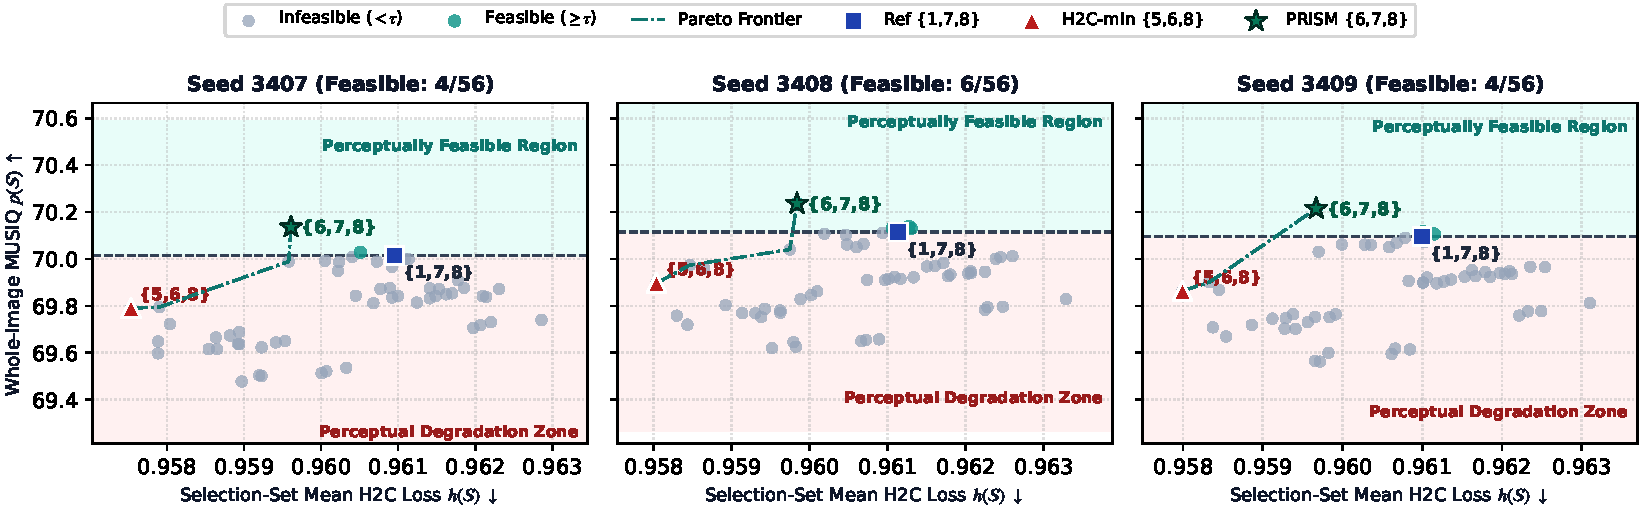
\includegraphics[width=0.95\textwidth]{figures/fig_landscape_en.pdf}
\caption{Measured 56-subset Level-3 feasibility landscape at shared epoch-5 snapshot $\theta_5$ across three seeds. Dashed line marks reference threshold $\tau=p(\mathcal{S}_{\rm ref})$. Unconstrained H2C minimization ($\{5,6,8\}$, triangles) falls below $\tau$, whereas \method~selects $\{6,7,8\}$ (stars) on all three seeds.}
\label{fig:landscape}
\end{figure*}
Figure~\ref{fig:landscape} plots all 56 Level-3 subsets in the $(\ell(\mathcal{S}),p(\mathcal{S}))$ plane across all three seeds. Without perceptual constraints, H2C minimization invariably selects $\{5,6,8\}$ (triangles; $\ell=0.95753$ on seed 3407), dropping whole-image MUSIQ below reference placement $\mathcal{S}_{\rm ref}=\{1,7,8\}$ ($\tau=70.015/70.115/70.096 \to 69.790/69.897/69.863$). \method~solves the discrete guardrail-constrained selection:
\begin{equation}
\mathcal{S}^\star=\underset{\substack{\mathcal{S}\subset\mathcal{I}\\|\mathcal{S}|=b}}{\arg\min}\ell(\mathcal{S})
\quad\text{s.t.}\quad p(\mathcal{S})\ge\tau,\quad \tau=p(\mathcal{S}_{\rm ref}),
\label{eq:selection}
\end{equation}
with lexicographical tie-breaking. Only 4/56 (7.1\%), 6/56 (10.7\%), and 4/56 (7.1\%) subsets satisfy $p(\mathcal{S})\ge\tau$ across seeds 3407--3409, and Eq.~\eqref{eq:selection} \textbf{converges consistently to $\mathcal{S}^\star=\{6,7,8\}$ on every seed}---which on $\mathcal{D}_{\rm sel}$ also coincides with the global MUSIQ maximum across all 56 subsets ($70.136/70.236/70.215$, outperforming $\{5,6,8\}$ by $+0.346/+0.339/+0.352$). We explicitly dissect this coincidence in Section~\ref{sec:ablation}.

\para{Phase-2 Fine-Tuning \& Lossless Reparameterization.}
Following selection, \method~extracts the 15 trainable tensors of $\mathcal{S}^\star$ (6 pairs of $A,B$ factors and 3 block gates, 110,595 params) from $\theta_5$, discards the remaining 13 blocks and bi-level architecture optimizer, resets a shared phase-2 RNG seed with a fresh Adam optimizer, and fine-tunes for 25 epochs under the unmodified H2C objective. Gradient-free probing takes $\sim$0.93\,s per subset ($\sim$52\,s total on an RTX 4090D). After fine-tuning, linearly folding the 6 LoRA deltas back into the base $3\times 3$ kernels yields exact deployment weights $W'$ matching baseline FLOPs, verified across all 3 seeds on smoke input \texttt{AM\_Bing\_211.png} with 0.0 max float error and 0\,LSB uint8 pixel error (Appendix~A.2, Algorithm~\ref{alg:prism}).

\begin{algorithm}[t]
\caption{\method: Perceptually Regulated Snapshot Masking}
\label{alg:prism}
\begin{algorithmic}[1]
\Require Frozen backbone $W$, training set $\mathcal{D}_{\rm tr}$, selection set $\mathcal{D}_{\rm sel}$, budget $b=3$
\State Estimate patch covariance on 32 calibration images; initialize $A_0=DV_d^\top, B_0=0$ on 16 candidate blocks (Eq.~\ref{eq:init})
\State Warm up all 16 BiLaLoRA candidate blocks jointly for 5 epochs via bi-level optimization to obtain shared snapshot $\theta_5$
\For{$\mathcal{S}\subset\mathcal{I}_{\rm L3}$ with $|\mathcal{S}|=b$ (56 equal-capacity Level-3 subsets)}
\State Evaluate $\ell(\mathcal{S})$ and $p(\mathcal{S})$ on $\mathcal{D}_{\rm sel}$ at $\theta_5$ without gradients (Eq.~\ref{eq:probe})
\EndFor
\State Set guardrail $\tau=p(\mathcal{S}_{\rm ref})$ and solve Eq.~\eqref{eq:selection} for $\mathcal{S}^\star$
\State Extract $\mathcal{S}^\star$ tensors (110,595 params), discard remaining 13 blocks, reset phase-2 seed/Adam, and fine-tune 25 epochs under H2C
\State \Return Zero-overhead merged model $W'$ via Eq.~\eqref{eq:lora}
\end{algorithmic}
\end{algorithm}

\section{Experiments}
\subsection{Experimental Setup \& Leakage-Free Protocol}
\para{Data Splits \& Deduplication Audit.}
Unpaired adaptation uses 500 public daytime real hazy images under a strict half-split partition: the first 250 images serve adapter weight updates, and the remaining 250 form the validation pool. Conv-EVA covariance statistics use 32 fixed images from the training half, while epoch-5 56-subset probing uses 32 non-overlapping images from the validation half. Primary quantitative evaluation spans \rtts~\cite{reside2019} ($n=4322$) and \fattal~\cite{fattal2014} ($n=31$); controlled ablations and severe-haze diagnostics evaluate \rttssub~(128 images sampled under fixed seed 20261123 from the remaining 1,850 RTTS pool outside pilot runs) and paired \dense~\cite{dense2019} ($n=55$, long edge capped at 800\,px). Per-image decoded SHA256 auditing confirms zero pixel overlap between the 500 adaptation images and RTTS; in Fattal, only \texttt{flags\_input.png} matches validation image \texttt{flag.jpg} (excluded from both training and $\mathcal{D}_{\rm sel}$), and Appendix~B provides an $n=30$ deduplicated sensitivity check confirming identical gains.

\para{Training Configuration \& Lossless Evaluation.}
All models start from pretrained DEA-Net (3,653,377 parameters) and train across three independent seeds (3407, 3408, 3409) with batch size 24, $224\times 224$ random crops, and learning rate $2\times 10^{-5}$ for $5+25$ epochs (locking post-snapshot augmentations and batch order identically across selection rules). All self-evaluated checkpoints output lossless uint8 PNGs via official normalization and 16-multiple bicubic resizing, scored uniformly on identical decoded pixels using FADE~\cite{fade2015} ($\downarrow$), BIQME~\cite{biqme2018} ($\uparrow$), KonIQ-weighted~\cite{koniq2020} MUSIQ~\cite{musiq2021} ($\uparrow$), and NIQE~\cite{niqe2013} ($\downarrow$) over fixed computable sets (complete audit details and symbols in Appendix~A.3).

\subsection{Main Benchmark Comparisons}
\begin{table*}[t]
\centering\small\setlength{\tabcolsep}{2.5pt}
\begin{tabular*}{\textwidth}{@{\extracolsep{\fill}}lrrrrrr@{}}\toprule
\multirow{2}{*}{Method} & \multicolumn{3}{c}{RTTS ($n=4322$)} & \multicolumn{3}{c}{Fattal ($n=31$)} \\
 & FADE$\downarrow$ & BIQME$\uparrow$ & MUSIQ$\uparrow$ & FADE$\downarrow$ & BIQME$\uparrow$ & MUSIQ$\uparrow$ \\\midrule
MSBDN~\cite{msbdn2020}$^\dagger$ & 1.483 & 0.549 & 52.93 & 0.613 & 0.555 & 63.71 \\
DeHamer~\cite{dehamer2022}$^\dagger$ & 1.806 & 0.542 & 52.90 & 0.756 & 0.552 & 64.31 \\
C2PNet~\cite{c2p2023}$^\dagger$ & 2.050 & 0.531 & 54.18 & 0.720 & 0.551 & 65.00 \\
DEA~\cite{dea2024}$^\dagger$ & 1.781 & 0.541 & 53.13 & 0.696 & 0.557 & 64.23 \\
PromptIR~\cite{promptir2023}$^\dagger$ & 1.765 & 0.546 & 53.80 & 0.668 & 0.558 & 64.96 \\
DiffUIR~\cite{diffuir2024}$^\dagger$ & 2.132 & 0.531 & 54.81 & 0.871 & 0.537 & 64.95 \\
MoCE-IR~\cite{moce2025}$^\dagger$ & 1.922 & 0.539 & 54.21 & 0.678 & 0.557 & 65.01 \\
FoundIR~\cite{foundir2025}$^\dagger$ & 1.760 & 0.553 & 54.96 & 0.759 & 0.560 & 65.83 \\
DAD~\cite{dad2020}$^\dagger$ & 1.131 & 0.561 & 49.34 & 0.487 & 0.589 & 59.38 \\
PSD~\cite{psd2021}$^\dagger$ & 1.143 & 0.524 & 52.81 & 0.438 & 0.554 & 63.80 \\
D4~\cite{d42022}$^\dagger$ & 1.404 & 0.556 & 53.57 & 0.457 & 0.537 & 64.14 \\
RIDCP~\cite{ridcp2023}$^\dagger$ & 0.955 & 0.600 & 59.14 & 0.396 & 0.604 & 66.10 \\
KANet~\cite{kanet2024}$^\dagger$ & 0.870 & 0.583 & 54.54 & 0.338 & 0.560 & 65.35 \\
CoA~\cite{coa2025}$^\dagger$ & 0.859 & 0.593 & 53.43 & 0.314 & 0.618 & 63.38 \\
IPC~\cite{ipc2025}$^\dagger$ & 1.105 & 0.592 & 59.61 & 0.368 & 0.593 & 67.58 \\
PHATNet~\cite{phatnet2025}$^\dagger$ & 0.845 & 0.585 & 56.43 & 0.331 & 0.604 & 66.87 \\
BiLaLoRA~\cite{bilalora2026}$^\dagger$ & 0.752 & 0.611 & \runnerup{61.77} & \runnerup{0.281} & 0.607 & 67.92 \\
\midrule
BiLaLoRA (Official) & 0.7544 & 0.6107 & \runnerup{61.77} & 0.3070 & 0.6206 & \best{68.59} \\
\midrule
Ref. \{1,7,8\}+EVA & \runnerup{\sd{0.7172}{0.0078}} & \runnerup{\sd{0.6112}{0.0008}} & \sd{61.65}{0.14} & \sd{0.2847}{0.0009} & \runnerup{\sd{0.6217}{0.0004}} & \sd{67.71}{0.09} \\
\method & \best{\sd{0.6241}{0.0055}} & \best{\sd{0.6191}{0.0002}} & \best{\sd{61.79}{0.05}} & \best{\sd{0.2714}{0.0019}} & \best{\sd{0.6248}{0.0003}} & \runnerup{\sd{68.02}{0.01}} \\
\bottomrule\end{tabular*}

\caption{Quantitative comparison across all 20 methods on RTTS ($n=4322$) and Fattal ($n=31$). $\dagger$ denotes results quoted from~\cite{bilalora2026}; self-evaluated rows run under unified lossless uint8 PNG decoding, with the bottom two rows reporting 3-seed mean$\pm$std. \best{Red bold} and \runnerup{blue underline} indicate best and second-best per column. Extended tables with Entropy, 2,000-bootstrap 95\% CIs, and $n=30$ screening appear in Appendix~B.}
\label{tab:main}
\end{table*}

We first confirm measurement consistency: re-evaluating the official merged BiLaLoRA weights on RTTS yields MUSIQ 61.77, BIQME 0.6107, and FADE 0.7544, closely aligning with published numbers (61.77, 0.611, 0.752). Against 20 methods across synthetically supervised backbones (MSBDN, DeHamer, C2PNet, DEA-Net), all-in-one restoration models (PromptIR, DiffUIR, MoCE-IR, FoundIR), full-network unpaired methods (DAD through PHATNet), and PEFT adapters (Table~\ref{tab:main}), \method~delivers strong dehazing gains at zero added inference cost:
\begin{itemize}\setlength{\itemsep}{1pt}\setlength{\parskip}{0pt}
\item \textbf{RTTS ($n=4322$)}: \method~leads FADE ($0.6241\pm 0.0055$), BIQME ($0.6191\pm 0.0002$), and MUSIQ ($61.79\pm 0.05$). Specifically, FADE drops by \textbf{13.0\%} over iso-budget matched-protocol Ref.~\(\{1,7,8\}\)+EVA (isolating the net gain of layer allocation) and by \textbf{17.0\%} over reported BiLaLoRA (0.752; 17.3\% over unified re-evaluation 0.7544), while MUSIQ cross-seed std drops from 0.14 to \textbf{0.05}.
\item \textbf{Fattal ($n=31$)}: \method~achieves the lowest FADE ($0.2714\pm 0.0019$, $-11.6\%$ vs. official BiLaLoRA 0.3070) and highest BIQME ($0.6248\pm 0.0003$). Official BiLaLoRA retains higher MUSIQ (68.59 vs. 68.02) at the cost of heavier residual haze (0.3070 vs. 0.2714), while \method~exceeds reported BiLaLoRA (67.92) and matched Ref.~\(\{1,7,8\}\)+EVA (67.71).
\end{itemize}

\para{Cross-Paradigm Perspective \& Paired Significance.}
Heavy supervised backbones and all-in-one models retain severe RTTS haze under domain shift (FADE 1.760--2.132, Entropy $\le 7.275$), whereas updating 3.03\% parameters in phase 2 enables \method~to outperform full-network unpaired methods while also leading RTTS Entropy (7.5799, Appendix Table~B.1). Across 30,471 main-table predictions (7 checkpoints $\times$ 4,353 RTTS+Fattal images), 2,000 image-paired bootstrap resamples (seed 20261115) against Ref.~\(\{1,7,8\}\)+EVA (Appendix Table~B.2) yield RTTS $\Delta\mathrm{FADE}=-0.0931$ (95\% CI $[-0.0955,-0.0909]$, \textbf{99.7\%} per-image win rate), $\Delta\mathrm{BIQME}=+0.0079$ (78.9\% win rate), and $\Delta\mathrm{MUSIQ}=+0.14$ ($[+0.10,+0.18]$), with all Fattal ($n=31$ and $n=30$) CIs strictly excluding zero ($>91\%$ FADE win rates).

\subsection{Rule Ablation, Sensitivity \& Trade-offs}
\label{sec:ablation}
\begin{table*}[t]
\centering\small\setlength{\tabcolsep}{2pt}
\begin{tabular*}{\textwidth}{@{\extracolsep{\fill}}lrrrrrr@{}}\toprule
\multirow{2}{*}{Selection Rule} & \multicolumn{3}{c}{RTTS-128 ($n=128$)} & \multicolumn{3}{c}{Dense-Haze ($n=55$)} \\
 & FADE$\downarrow$ & MUSIQ$\uparrow$ & NIQE$\downarrow$ & FADE$\downarrow$ & MUSIQ$\uparrow$ & NIQE$\downarrow$ \\\midrule
Reference \{1,7,8\} & \sd{0.6991}{0.0074} & \sd{62.26}{0.15} & \sd{4.90}{0.02} & \sd{0.7475}{0.0025} & \best{\sd{54.80}{0.06}} & \sd{5.41}{0.02} \\
H2C-min \{5,6,8\} & \best{\sd{0.6122}{0.0145}} & \sd{61.18}{0.14} & \best{\sd{4.64}{0.02}} & \best{\sd{0.5822}{0.0213}} & \sd{52.65}{0.25} & \best{\sd{4.72}{0.04}} \\
Restricted Gate & \sd{0.6435}{0.0474} & \runnerup{\sd{62.28}{0.54}} & \runnerup{\sd{4.88}{0.02}} & \sd{0.6544}{0.0339} & \sd{53.24}{0.58} & \runnerup{\sd{4.99}{0.18}} \\
\method~\{6,7,8\} & \runnerup{\sd{0.6147}{0.0053}} & \best{\sd{62.57}{0.05}} & \runnerup{\sd{4.88}{0.02}} & \runnerup{\sd{0.6343}{0.0036}} & \runnerup{\sd{53.58}{0.05}} & \sd{5.09}{0.05} \\
\bottomrule\end{tabular*}

\caption{Controlled ablation of discrete selection rules from shared $\theta_5$ under equal phase-2 capacity ($b=3$, $110{,}595$ trainable parameters) and identical 25-epoch streams (3-seed mean$\pm$std). Restricted Gate selects $\{6,7,8\}$, $\{2,6,8\}$, $\{6,7,8\}$ on seeds 3407--3409.}
\label{tab:ablation}
\end{table*}
Table~\ref{tab:ablation} evaluates four discrete selection rules starting from the same $\theta_5$, 3.03\% phase-2 budget, and 25-epoch stream:
\begin{enumerate}\setlength{\itemsep}{1pt}\setlength{\parskip}{0pt}
\item \textbf{Semantic--Perceptual Mismatch}: Minimizing H2C alone reliably picks $\{5,6,8\}$, attaining the lowest FADE (0.6122 / 0.5822) at the expense of whole-image MUSIQ degradation (61.18 on RTTS-128, 52.65 on Dense-Haze---trailing \method~by 1.39 and 0.93 points). Local high-frequency-driven NIQE still favors over-sharpened $\{5,6,8\}$, highlighting why whole-image MUSIQ is critical for selection. Meanwhile, \method~cuts RTTS-128 FADE by 12.1\% below Ref.~\(\{1,7,8\}\) ($0.6991 \to 0.6147$) while achieving the highest group MUSIQ (\textbf{62.57}).
\item \textbf{Restricted vs. Unrestricted Gating}: Unrestricted 16-block gating diverges across all three seeds into shallow encoder blocks (RTTS-128 FADE std 0.0507 for \texttt{baseline\_dynamic} and 0.1304 for \texttt{eva\_dynamic}, collapsing capacity to 55,299 params on seed 3409). Even after restricting top-3 gates to the 8 equal-capacity Level-3 blocks (Table~\ref{tab:ablation}), gate ranking still diverges once on seed 3408 ($\{6,7,8\}$, $\{2,6,8\}$, $\{6,7,8\}$, sharing the 3407/3409 models with \method), giving RTTS-128 FADE std 0.0474 (vs. \method's \textbf{0.0053}) and Dense-Haze std 0.0339 (vs. \textbf{0.0036}).
\item \textbf{Attribution: Two-Step Guardrail vs. Direct $\arg\max$ MUSIQ}: On $\mathcal{D}_{\rm sel}$ (3 seeds, 8 Level-3 blocks), $\{6,7,8\}$ is both the feasible H2C minimum and the global MUSIQ maximum, so the current 3-seed main table reflects whole-image quality-guided selection rather than isolating the two-step rule from single-step $\arg\max\mathrm{MUSIQ}$. To test separability directly, we ran an auxiliary 1,232-subset epoch-5 probe across 32-image \texttt{RTTS-128} and \texttt{Dense-Haze} splits (both 8-block and full 16-block 560-subset spaces): (i) expanding to all 16 blocks causes both min-H2C and two-step selection on RTTS to collapse into pure shallow \texttt{down\_level1} blocks (27,651 params, worse snapshot FADE 1.1500 vs. 1.1286), validating our iso-budget Level-3 restriction; (ii) on the 32-image \texttt{RTTS-128} Level-3 split (seed 3407), the fixed reference guardrail $\tau$ slightly leaks $\{5,6,8\}$ (62.497 $\ge$ 62.477), whereas direct $\arg\max\mathrm{MUSIQ}$ still locks $\{6,7,8\}$---and evaluating existing matched 30-epoch checkpoints on the remaining 96 held-out \texttt{RTTS-128} images confirms $\{6,7,8\}$ retains $+1.24$ higher MUSIQ (61.68 vs. 60.44) at comparable FADE (0.6255 vs. 0.6236). Thus, equal-capacity Level-3 scoping and whole-image perceptual scoring are the primary effective drivers, while adaptive guardrail calibration remains an important avenue for future work.
\end{enumerate}

\para{Efficiency \& Stability Trade-off.}
Appendix Figure~\ref{fig:bubble}(a) places all methods on the $256\times 256$ FLOPs vs. RTTS FADE plane. Heavy backbones consume tens of millions of parameters and hundreds of GFLOPs (e.g., C2PNet 460.9G, DeHamer 132.4M) yet stagnate at FADE 1.48--2.13. After lossless linear merging, BiLaLoRA, Ref.~\(\{1,7,8\}\), and \method~all share DEA-Net's exact \textbf{3.65M} parameters and \textbf{32.23G} FLOPs, while \method~pushes FADE vertically down to 0.6241. Panel~(b) contrasts cross-seed FADE std against RTTS-128 MUSIQ (0.0053 vs. 0.0474 for restricted gating).

\subsection{Qualitative Comparisons \& Spatial Modulation}
\begin{figure*}[t]
\centering\setlength{\tabcolsep}{2pt}\begin{tabular}{ccccc}
Hazy Input & BiLaLoRA (Official) & Ref. \{1,7,8\}+EVA & \method & $8\times$ Diff. \\
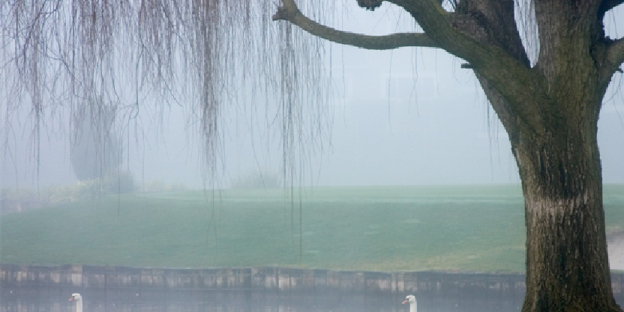
\includegraphics[width=.188\textwidth]{figures/swan_input_crop.png} & 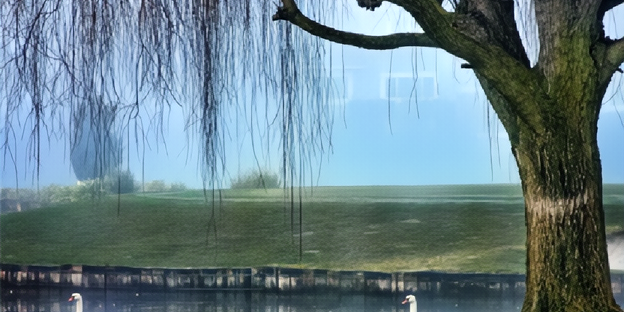
\includegraphics[width=.188\textwidth]{figures/swan_official_bilalora_crop.png} & 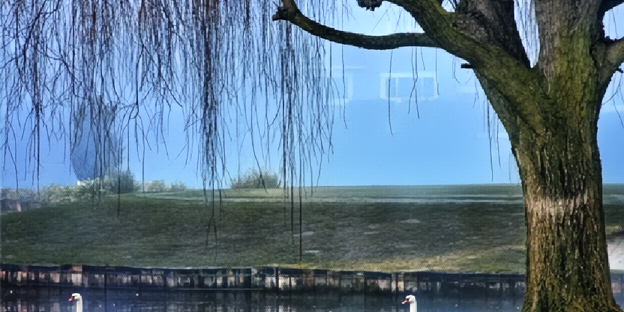
\includegraphics[width=.188\textwidth]{figures/swan_warm_published_3407_crop.png} & 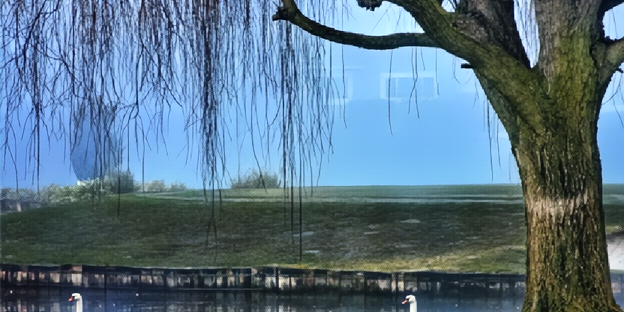
\includegraphics[width=.188\textwidth]{figures/swan_warm_quality_constrained_3407_crop.png} & 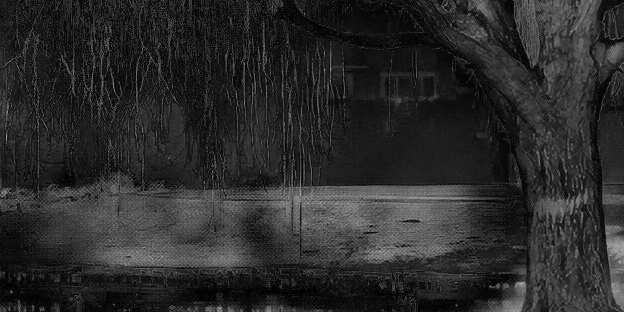
\includegraphics[width=.188\textwidth]{figures/swan_difference.png} \\
\footnotesize {\footnotesize \texttt{swan}} & {\footnotesize 0.3081 / 71.14} & {\footnotesize 0.2503 / 70.52} & {\footnotesize \best{0.2423} / \best{71.97}} & {\footnotesize $\Delta$MUSIQ=+1.45} \\[5pt]
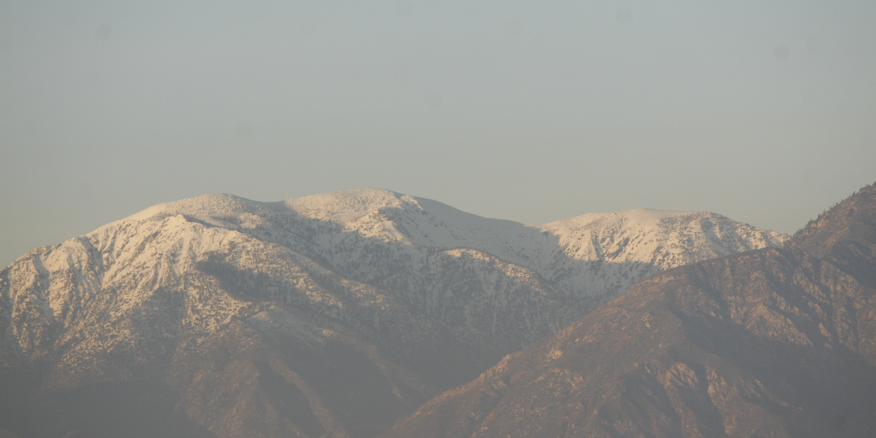
\includegraphics[width=.188\textwidth]{figures/snow_input_crop.png} & 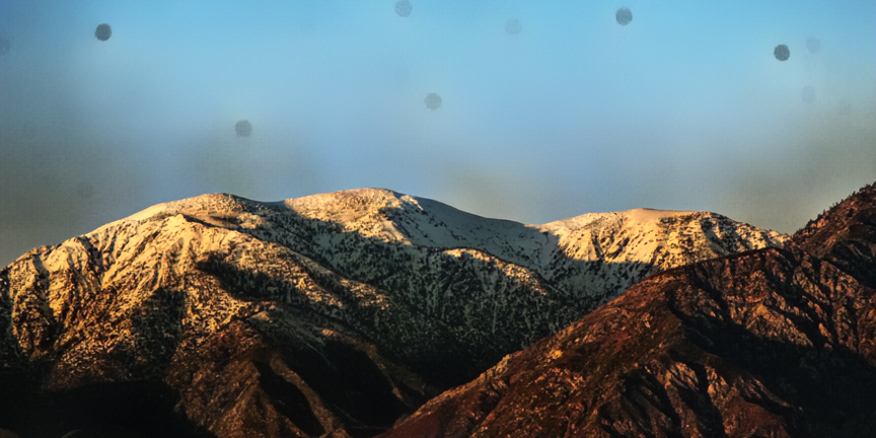
\includegraphics[width=.188\textwidth]{figures/snow_official_bilalora_crop.png} & 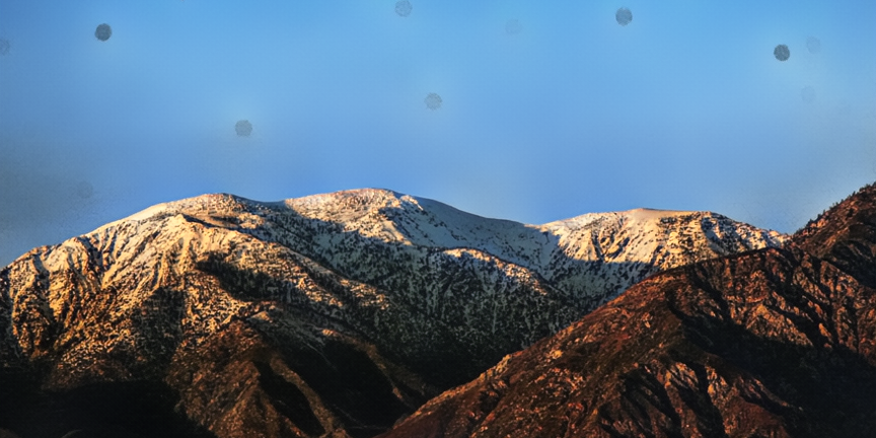
\includegraphics[width=.188\textwidth]{figures/snow_warm_published_3407_crop.png} & 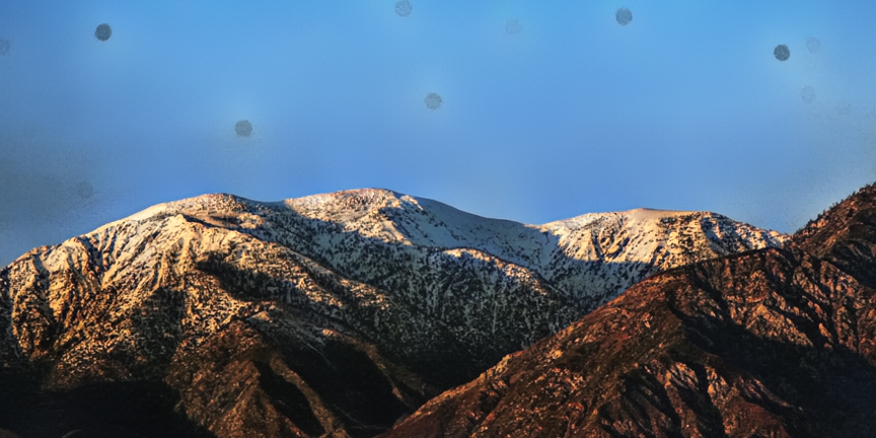
\includegraphics[width=.188\textwidth]{figures/snow_warm_quality_constrained_3407_crop.png} & 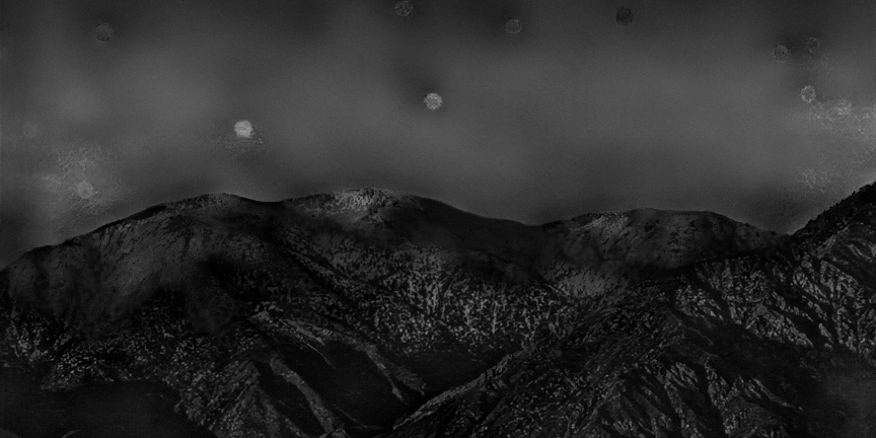
\includegraphics[width=.188\textwidth]{figures/snow_difference.png} \\
\footnotesize {\footnotesize \texttt{snow}} & {\footnotesize 0.7007 / 65.42} & {\footnotesize 0.6558 / 67.45} & {\footnotesize \best{0.6231} / \best{68.23}} & {\footnotesize $\Delta$MUSIQ=+0.79} \\[5pt]
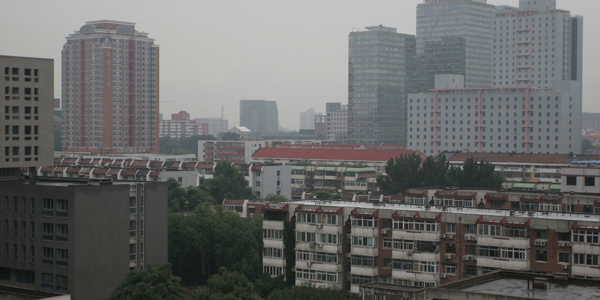
\includegraphics[width=.188\textwidth]{figures/buildings_input_crop.png} & 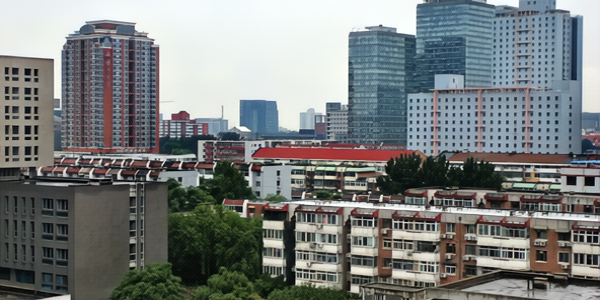
\includegraphics[width=.188\textwidth]{figures/buildings_official_bilalora_crop.png} & 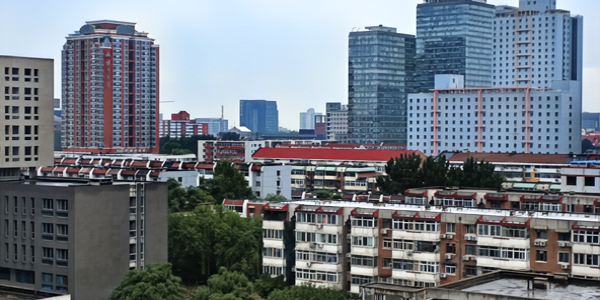
\includegraphics[width=.188\textwidth]{figures/buildings_warm_published_3407_crop.png} & 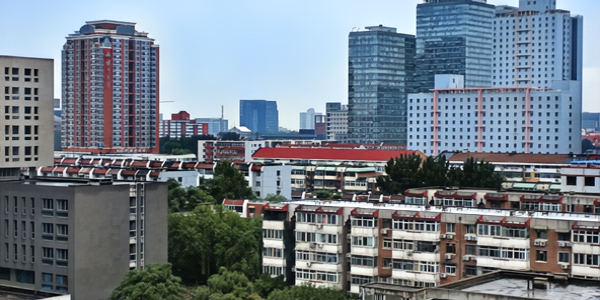
\includegraphics[width=.188\textwidth]{figures/buildings_warm_quality_constrained_3407_crop.png} & 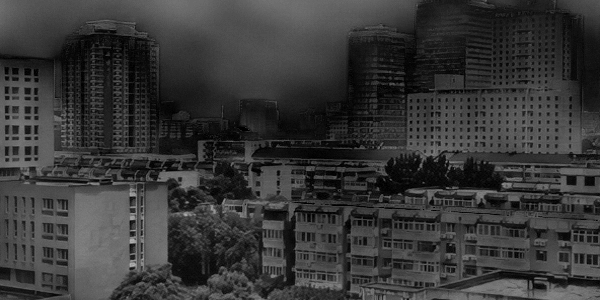
\includegraphics[width=.188\textwidth]{figures/buildings_difference.png} \\
\footnotesize {\footnotesize \texttt{buildings}} & {\footnotesize 0.4828 / 69.91} & {\footnotesize 0.4109 / 70.21} & {\footnotesize \best{0.3934} / \best{70.84}} & {\footnotesize $\Delta$MUSIQ=+0.62} \\[5pt]
\end{tabular}

\caption{Aligned $2:1$ qualitative comparisons on Fattal scenes (seed 3407; whole-image FADE$\downarrow$ / MUSIQ$\uparrow$ below) and $8\times|\mathrm{PRISM}-\mathrm{Ref}|$ spatial differences. \method~targets distant scattering regions selectively while preserving natural foreground tone.}
\label{fig:visual}
\end{figure*}
Figure~\ref{fig:visual} presents $2:1$ aligned detail crops and $8\times|\mathrm{\method}-\mathrm{Ref}|$ spatial difference maps across \texttt{swan}, \texttt{snow}, and \texttt{buildings} (seed 3407). Two consistent patterns emerge: (1) \method~clears distant atmospheric veiling that lingers in official BiLaLoRA outputs---recovering crisp glass facades and sky gradients in \texttt{buildings} (FADE $0.4828 \to \best{0.3934}$, MUSIQ \best{70.84}) and sharp mountain ridgelines in \texttt{snow} (FADE \best{0.6231}, MUSIQ \best{68.23}); (2) the $8\times$ difference maps show that relative to Ref.~\(\{1,7,8\}\)+EVA, \method~concentrates corrective modulation onto distant scattering layers and high-contrast structures rather than indiscriminately over-sharpening foreground water in \texttt{swan} (lifting MUSIQ $70.52 \to \best{71.97}$, netting $+0.62$ to $+1.45$ MUSIQ across the three scenes). Uncropped full-aspect qualitative views of these Fattal scenes and an analysis of the Fattal \texttt{train} boundary case appear in Appendix~D.

\subsection{Decoupling Verification \& Severe-Fog Diagnostics}
\label{sec:exp_diagnostic}
\begin{table}[!htbp]
\centering\footnotesize\setlength{\tabcolsep}{1.6pt}
\resizebox{\columnwidth}{!}{\begin{tabular*}{\textwidth}{@{\extracolsep{\fill}}lrrrr@{}}\toprule
\multicolumn{5}{l}{\textbf{(a) Score Supervision Location and Scale: Fixed \{5,6,8\}, 30+5 Epochs}} \\
\multirow{2}{*}{Training Objective} & \multicolumn{2}{c}{RTTS-128 ($n=128$)} & \multicolumn{2}{c}{Dense-Haze ($n=55$)} \\
 & FADE$\downarrow$ & MUSIQ$\uparrow$ & FADE$\downarrow$ & MUSIQ$\uparrow$ \\\midrule
H2C Only & \sd{0.5493}{0.0077} & \sd{61.60}{0.21} & \sd{0.5341}{0.0184} & \sd{53.51}{0.29} \\
H2C + Crop Score & \sd{0.5788}{0.0060} & \sd{61.86}{0.18} & \sd{0.5701}{0.0193} & \sd{53.67}{0.11} \\
H2C + Full-224 Score & \sd{0.5572}{0.0056} & \sd{61.48}{0.15} & \sd{0.5410}{0.0128} & \sd{52.94}{0.17} \\
H2C + Full-1024 Score & \sd{0.5899}{0.0088} & \sd{62.23}{0.25} & \sd{0.5863}{0.0254} & \sd{54.44}{0.24} \\
\midrule\multicolumn{5}{l}{\textbf{(b) Severe-Fog Domain Diagnostic: Shared Snapshot, 5+25 Epochs}} \\
Selection Rule & PSNR$\uparrow$ & SSIM$\uparrow$ & FADE$\downarrow$ & MUSIQ$\uparrow$ \\\midrule
Reference \{1,7,8\} & \sd{11.9296}{0.0409} & \sd{0.5101}{0.0014} & \sd{0.7475}{0.0025} & \sd{54.80}{0.06} \\
\method~\{6,7,8\} & \sd{12.2210}{0.0366} & \sd{0.5063}{0.0011} & \sd{0.6343}{0.0036} & \sd{53.58}{0.05} \\
\bottomrule\end{tabular*}
}
\caption{Train--probe decoupling diagnostics and severe-fog evaluation (3-seed mean$\pm$std). \textbf{(a)} 5-epoch continuation from epoch-30 $\{5,6,8\}$ comparing unmodified H2C against multi-scale direct MUSIQ backpropagation; \textbf{(b)} zero-shot generalization on Dense-Haze ($n=55$). Full 5-metric tables and boundary case \texttt{train} appear in Appendix~B and Appendix~D.}
\label{tab:extension}
\end{table}

\para{Failure Modes of Direct Perceptual Backpropagation.}
Table~\ref{tab:extension}(a) (detailed across all 5 metrics in Appendix Table~B.5) confirms why perceptual scores should not enter gradient backpropagation directly. Continuing from the same epoch-30 $\{5,6,8\}$ state for 5 epochs: (1) backpropagating $224\times 224$ random-crop MUSIQ degrades dehazing due to missing global framing (RTTS-128 FADE $0.5493 \to 0.5788$; Dense-Haze $0.5341 \to 0.5701$); (2) aspect-preserving max-edge-224 whole-image MUSIQ backprop lowers MUSIQ itself on both benchmarks ($61.60 \to 61.48$; $53.51 \to 52.94$); and (3) pushing max-edge to 1024 raises MUSIQ (62.23 / 54.44) at the cost of sharply weakened dehazing ($+0.0406$ and $+0.0522$ FADE rebound) and heavy memory usage. Restricting MUSIQ to gradient-free snapshot probing cleanly avoids this optimization shortcut.

\para{Severe-Fog Transfer \& Perception--Distortion Boundary.}
On unseen paired Dense-Haze ($n=55$, Table~\ref{tab:extension}(b)), \method~improves full-reference fidelity \textbf{PSNR by +0.2914\,dB} ($11.9296 \to 12.2210$) and cuts \textbf{FADE by 15.1\%} ($0.7475 \to 0.6343$) relative to Ref.~\(\{1,7,8\}\), validating deep bottleneck efficacy under heavy physical scattering. Uncovering dense dark gravel and shadowed backgrounds trades off against KonIQ-MUSIQ ($54.80 \to 53.58$) and slightly lowers SSIM ($0.5101 \to 0.5063$), aligning with the perception--distortion frontier~\cite{perception2018} and our \texttt{train} boundary analysis in Appendix~D.

\section{Conclusion}
We presented \method, a decoupled probing--training framework that introduces whole-image perceptual evaluation into budget-constrained low-rank layer selection for unpaired real-world dehazing. By uniting Conv-EVA initialization and BiLaLoRA's 5-epoch 16-block warm-up with gradient-free 56-subset iso-budget Level-3 probing, \method~consistently selects $\{6,7,8\}$ across all three seeds without modifying the H2C fine-tuning objective. After lossless linear reparameterization, updating 3.03\% parameters reduces RTTS ($n=4322$) FADE by 13.0\% over matched-protocol reference placement (17.0\% over reported BiLaLoRA) at identical baseline FLOPs, while transparently revealing perception--distortion trade-offs on Fattal and Dense-Haze as well as threshold sensitivity relative to direct MUSIQ maximization. Future work will explore adaptive perceptual thresholds, dynamic rank allocation, and temporally consistent video dehazing.

\para{LLM Usage Statement.}
Large language models were used solely to assist with English wording polish, LaTeX formatting, and auxiliary plotting/audit script organization; all experimental design, model execution, statistical verification, and scientific claims were independently checked and verified by the authors.

\FloatBarrier
{\small\interlinepenalty=10000\bibliographystyle{ieeenat_fullname}\bibliography{references,references_extra}}

% ==============================================================================
% UNIFIED APPENDIX (A-D) IN CLEAN SINGLE-COLUMN FORMAT
% ==============================================================================
\clearpage
\onecolumn
\appendix
\counterwithin{table}{section}
\counterwithin{figure}{section}
\setcounter{table}{0}
\setcounter{figure}{0}

\section{Implementation \& Verification Details}
\subsection{Conv-EVA Zero-Drift Initialization}
Let $W_{\rm mat}=\mathcal{R}(W)\in\mathbb{R}^{(c_o\kappa)\times(c_i\kappa)}$ denote the unfolded kernel matrix of an adapted $3\times 3$ convolution across BiLaLoRA's 16 candidate blocks (\texttt{down\_level1}: $c=32$, \texttt{down\_level2}: $c=64$, \texttt{level3}: $c=128$). By Eqs.~\eqref{eq:lora} and~\eqref{eq:init}, initial weight increment obeys $\Delta W_0=\gamma g_0\,\mathcal{R}^{-1}(B_0 A_0)$. Setting $B_0=0$ guarantees $\Delta W_0\equiv 0$ regardless of $A_0$ or $\gamma$, preserving exact pretrained DEA-Net outputs at epoch 0. Sampling up to 256 unfolded patch locations per image across 32 real hazy training images ($N=24{,}576$ unfolded rows aligned with $\mathcal{R}$), Conv-EVA computes the centered activation covariance $\Sigma=\frac{1}{N}\tilde{X}^\top\tilde{X}=V\Lambda V^\top$ and initializes $A_0=DV_d^\top$ along the top $d=r\kappa=24$ eigenvectors while retaining each row's original Kaiming $\ell_2$ norm ($D_{jj}=\|(A_{\rm rand})_j\|_2$). This provides a deterministic, data-aligned starting subspace across all 16 blocks prior to the 5-epoch warm-up without making uniformity assumptions on row scaling.

\subsection{Lossless Inference Reparameterization Verification}
Across selected Level-3 blocks $\mathcal{S}^\star=\{6,7,8\}$, the 6 adapted $3\times 3$ convolutions ($c_o=c_i=128,\kappa=3,r=8,d=24$) carry low-rank factors $(A,B)$ and block gates $g=\sigma(u_{\rm gate})$. Exploiting linearity of 2D convolution over kernel sums, evaluating $W' = W + \gamma g\,\mathcal{R}^{-1}(BA)$ once after fine-tuning merges all 3.03\% adapter weights into the base kernels and removes all LoRA wrappers (restoring exact base parameter count 3,653,377 and baseline FLOPs). Single-image smoke checks in \texttt{merge\_audit.json} across all three seeds (3407--3409) on \texttt{AM\_Bing\_211.png} confirm 0.0 maximum float output difference and 0\,LSB uint8 PNG difference before and after merging.

\subsection{Splits, SHA256 Deduplication Audit, \& Notation}
Adaptation uses 500 daytime hazy images partitioned equally into 250 training images (32 sampled for Conv-EVA) and 250 validation images (32 disjointly sampled for $\mathcal{D}_{\rm sel}$). Decoded SHA256 auditing shows zero pixel overlap between the 500-image set and RTTS ($n=4322$), and a single overlap in Fattal ($n=31$: \texttt{flags\_input.png} matches unused validation image \texttt{flag.jpg}), with $n=30$ deduplicated means in Table~\ref{tab:screen}. All metrics evaluate identical decoded PNG pixels including RGB 256-bin joint Shannon entropy~\cite{shannon1948} and fixed-computable NIQE (128 images on RTTS-128, 55 on Dense-Haze). Table~\ref{tab:symbols} summarizes all mathematical notation.

\begin{table}[H]\centering\small
\begin{tabular*}{0.92\textwidth}{@{\extracolsep{\fill}}ll@{}}\toprule
Symbol & Definition \& Dimension \\\midrule
$H,W$ & Input height and width (Level-3 bottleneck spatial size $H/4\times W/4$) \\
$c_i,c_o,\kappa$ & Input/output channels ($32/64/128$ across levels; $128$ in Level-3) and kernel size ($3$) \\
$\mathcal{R},\mathcal{R}^{-1}$ & Kernel unfolding operator $\mathbb{R}^{c_o\times c_i\times\kappa\times\kappa}\to\mathbb{R}^{(c_o\kappa)\times(c_i\kappa)}$ and inverse \\
$r,d$ & Adapter rank ($8$) and unfolded inner width ($d=r\kappa=24$) \\
$X,\Sigma$ & Unfolded activation matrix over 32 calibration images ($N=24{,}576$ rows) and centered covariance \\
$V_d,D$ & Top-$d$ eigenvectors of $\Sigma$ and diagonal Kaiming row-norm scaler \\
$\gamma,g$ & Fixed scaling factor ($\alpha_{\rm LoRA}/r=2$) and shared block sigmoid gate $\sigma(u_{\rm gate})$ \\
$\mathcal{S},\theta_5,b$ & Candidate Level-3 subset (budget $b=3$) and shared epoch-5 16-block warm-up snapshot \\
$\ell(\mathcal{S}),p(\mathcal{S}),\tau$ & Mean H2C loss on $\mathcal{D}_{\rm sel}$, deployment MUSIQ, and reference guardrail $p(\mathcal{S}_{\rm ref})$ \\\bottomrule
\end{tabular*}
\caption{Summary of mathematical notation used in the main text and appendices.}
\label{tab:symbols}
\end{table}

\clearpage
\section{Extended Benchmarks \& Statistical Significance Tests}
Table~\ref{tab:full} reports full 20-method comparisons including RGB joint entropy; Table~\ref{tab:effects} presents 2,000-iteration paired bootstrap intervals (seed 20261115); Table~\ref{tab:seeds} breaks down per-seed scores; Table~\ref{tab:screen} validates Fattal ($n=30$) after overlap removal; and Table~\ref{tab:diagfull} provides all 5 metrics for the multi-scale perceptual backpropagation diagnostic.

\begin{table}[H]\centering\small\setlength{\tabcolsep}{2.5pt}
\begin{tabular*}{\textwidth}{@{\extracolsep{\fill}}lrrrrrrrr@{}}\toprule
\multirow{2}{*}{Method} & \multicolumn{4}{c}{RTTS ($n=4322$)} & \multicolumn{4}{c}{Fattal ($n=31$)} \\
 & FADE$\downarrow$ & BIQME$\uparrow$ & Entropy$\uparrow$ & MUSIQ$\uparrow$ & FADE$\downarrow$ & BIQME$\uparrow$ & Entropy$\uparrow$ & MUSIQ$\uparrow$ \\\midrule
MSBDN~\cite{msbdn2020}$^\dagger$ & 1.483 & 0.549 & 7.273 & 52.93 & 0.613 & 0.555 & 7.408 & 63.71 \\
DeHamer~\cite{dehamer2022}$^\dagger$ & 1.806 & 0.542 & 7.215 & 52.90 & 0.756 & 0.552 & 7.411 & 64.31 \\
C2PNet~\cite{c2p2023}$^\dagger$ & 2.050 & 0.531 & 7.168 & 54.18 & 0.720 & 0.551 & 7.399 & 65.00 \\
DEA~\cite{dea2024}$^\dagger$ & 1.781 & 0.541 & 7.196 & 53.13 & 0.696 & 0.557 & 7.423 & 64.23 \\
PromptIR~\cite{promptir2023}$^\dagger$ & 1.765 & 0.546 & 7.189 & 53.80 & 0.668 & 0.558 & 7.498 & 64.96 \\
DiffUIR~\cite{diffuir2024}$^\dagger$ & 2.132 & 0.531 & 7.172 & 54.81 & 0.871 & 0.537 & 7.373 & 64.95 \\
MoCE-IR~\cite{moce2025}$^\dagger$ & 1.922 & 0.539 & 7.191 & 54.21 & 0.678 & 0.557 & 7.409 & 65.01 \\
FoundIR~\cite{foundir2025}$^\dagger$ & 1.760 & 0.553 & 7.275 & 54.96 & 0.759 & 0.560 & 7.376 & 65.83 \\
DAD~\cite{dad2020}$^\dagger$ & 1.131 & 0.561 & 7.413 & 49.34 & 0.487 & 0.589 & 7.487 & 59.38 \\
PSD~\cite{psd2021}$^\dagger$ & 1.143 & 0.524 & 7.276 & 52.81 & 0.438 & 0.554 & 7.463 & 63.80 \\
D4~\cite{d42022}$^\dagger$ & 1.404 & 0.556 & 7.179 & 53.57 & 0.457 & 0.537 & 7.372 & 64.14 \\
RIDCP~\cite{ridcp2023}$^\dagger$ & 0.955 & 0.600 & 7.541 & 59.14 & 0.396 & 0.604 & 7.468 & 66.10 \\
KANet~\cite{kanet2024}$^\dagger$ & 0.870 & 0.583 & 7.517 & 54.54 & 0.338 & 0.560 & 7.527 & 65.35 \\
CoA~\cite{coa2025}$^\dagger$ & 0.859 & 0.593 & \runnerup{7.579} & 53.43 & 0.314 & 0.618 & 7.585 & 63.38 \\
IPC~\cite{ipc2025}$^\dagger$ & 1.105 & 0.592 & 7.469 & 59.61 & 0.368 & 0.593 & 7.471 & 67.58 \\
PHATNet~\cite{phatnet2025}$^\dagger$ & 0.845 & 0.585 & 7.349 & 56.43 & 0.331 & 0.604 & 7.498 & 66.87 \\
BiLaLoRA~\cite{bilalora2026}$^\dagger$ & 0.752 & 0.611 & 7.576 & \runnerup{61.77} & \runnerup{0.281} & 0.607 & 7.541 & 67.92 \\
\midrule
BiLaLoRA (Official) & 0.7544 & 0.6107 & 7.5757 & \runnerup{61.77} & 0.3070 & 0.6206 & \best{7.6124} & \best{68.59} \\
\midrule
Ref. \{1,7,8\}+EVA & \runnerup{0.7172} & \runnerup{0.6112} & 7.5785 & 61.65 & 0.2847 & \runnerup{0.6217} & \runnerup{7.5992} & 67.71 \\
\method & \best{0.6241} & \best{0.6191} & \best{7.5799} & \best{61.79} & \best{0.2714} & \best{0.6248} & 7.5942 & \runnerup{68.02} \\
\bottomrule\end{tabular*}

\caption{Complete 20-method benchmark on RTTS ($n=4322$) and Fattal ($n=31$) including RGB joint entropy. $\dagger$ from~\cite{bilalora2026}; bottom two rows show 3-seed means. \best{Red bold}: best; \runnerup{blue underline}: second best.}
\label{tab:full}
\end{table}

\begin{table}[H]\centering\small\setlength{\tabcolsep}{3pt}
\begin{tabular*}{\textwidth}{@{\extracolsep{\fill}}llrrrr@{}}\toprule
Split & Metric & Mean $\Delta$ & Seed Std & Paired 95\% CI & Per-Image Win Rate \\\midrule
RTTS (4322) & FADE & -0.0931 & 0.0108 & $[-0.0955,-0.0909]$ & 99.7\% \\
RTTS (4322) & BIQME & +0.0079 & 0.0010 & $[0.0075,0.0083]$ & 78.9\% \\
RTTS (4322) & Entropy & +0.0014 & 0.0045 & $[-0.0013,0.0041]$ & 46.3\% \\
RTTS (4322) & MUSIQ & +0.14 & 0.09 & $[0.10,0.18]$ & 59.9\% \\
Fattal (31) & FADE & -0.0133 & 0.0024 & $[-0.0190,-0.0082]$ & 91.4\% \\
Fattal (31) & BIQME & +0.0031 & 0.0001 & $[0.0002,0.0057]$ & 73.1\% \\
Fattal (31) & Entropy & -0.0050 & 0.0017 & $[-0.0178,0.0126]$ & 34.4\% \\
Fattal (31) & MUSIQ & +0.31 & 0.08 & $[0.07,0.52]$ & 75.3\% \\
Fattal (30) & FADE & -0.0135 & 0.0024 & $[-0.0193,-0.0081]$ & 91.1\% \\
Fattal (30) & BIQME & +0.0033 & 0.0001 & $[0.0003,0.0059]$ & 75.6\% \\
Fattal (30) & Entropy & -0.0044 & 0.0017 & $[-0.0179,0.0136]$ & 35.6\% \\
Fattal (30) & MUSIQ & +0.30 & 0.08 & $[0.05,0.52]$ & 74.4\% \\
\bottomrule\end{tabular*}

\caption{Per-image paired differences between \method~(\{6,7,8\}) and iso-budget Ref.~\(\{1,7,8\}\)+EVA with 2,000-bootstrap (seed 20261115) 95\% CIs and win rates (lower FADE / higher BIQME, Entropy, MUSIQ count as improvements).}
\label{tab:effects}
\end{table}

\begin{table}[H]\centering\small\setlength{\tabcolsep}{3pt}
\begin{tabular*}{\textwidth}{@{\extracolsep{\fill}}llrrrr@{}}\toprule
Split & Model / Seed & FADE$\downarrow$ & BIQME$\uparrow$ & Entropy$\uparrow$ & MUSIQ$\uparrow$ \\\midrule
RTTS (4322) & Ref. / 3407 & 0.7142 & 0.6115 & 7.5786 & 61.75 \\
RTTS (4322) & Ref. / 3408 & 0.7261 & 0.6103 & 7.5764 & 61.49 \\
RTTS (4322) & Ref. / 3409 & 0.7113 & 0.6117 & 7.5805 & 61.71 \\
RTTS (4322) & \method / 3407 & 0.6304 & 0.6190 & 7.5793 & 61.82 \\
RTTS (4322) & \method / 3408 & 0.6212 & 0.6193 & 7.5826 & 61.73 \\
RTTS (4322) & \method / 3409 & 0.6207 & 0.6189 & 7.5778 & 61.81 \\
Fattal (31) & Ref. / 3407 & 0.2840 & 0.6215 & 7.5965 & 67.80 \\
Fattal (31) & Ref. / 3408 & 0.2858 & 0.6222 & 7.6026 & 67.63 \\
Fattal (31) & Ref. / 3409 & 0.2844 & 0.6215 & 7.5985 & 67.72 \\
Fattal (31) & \method / 3407 & 0.2735 & 0.6247 & 7.5933 & 68.04 \\
Fattal (31) & \method / 3408 & 0.2710 & 0.6252 & 7.5973 & 68.01 \\
Fattal (31) & \method / 3409 & 0.2698 & 0.6246 & 7.5919 & 68.01 \\
\bottomrule\end{tabular*}

\caption{Per-seed breakdown across seeds 3407, 3408, and 3409 on RTTS and Fattal.}
\label{tab:seeds}
\end{table}

\begin{table}[H]\centering\small\setlength{\tabcolsep}{4pt}
\begin{tabular*}{\textwidth}{@{\extracolsep{\fill}}lrrrr@{}}\toprule
Fattal ($n=30$) & FADE$\downarrow$ & BIQME$\uparrow$ & Entropy$\uparrow$ & MUSIQ$\uparrow$ \\\midrule
Ref. \{1,7,8\}+EVA & \sd{0.2891}{0.0010} & \sd{0.6213}{0.0004} & \sd{7.5907}{0.0032} & \sd{67.60}{0.09} \\
\method & \sd{0.2756}{0.0019} & \sd{0.6246}{0.0003} & \sd{7.5863}{0.0028} & \sd{67.90}{0.01} \\
\bottomrule\end{tabular*}

\caption{Sensitivity check on Fattal ($n=30$) after excluding \texttt{flags\_input.png} (3-seed mean$\pm$std).}
\label{tab:screen}
\end{table}

\begin{table}[H]\centering\small\setlength{\tabcolsep}{3pt}
\begin{tabular*}{\textwidth}{@{\extracolsep{\fill}}llrrrrr@{}}\toprule
Split & Training Objective & FADE$\downarrow$ & MUSIQ$\uparrow$ & NIQE$\downarrow$ & PSNR$\uparrow$ & SSIM$\uparrow$ \\\midrule
RTTS-128 & H2C Only & \sd{0.5493}{0.0077} & \sd{61.60}{0.21} & \sd{4.66}{0.03} & -- & -- \\
RTTS-128 & H2C + Crop Score & \sd{0.5788}{0.0060} & \sd{61.86}{0.18} & \sd{4.69}{0.03} & -- & -- \\
RTTS-128 & H2C + Full-224 Score & \sd{0.5572}{0.0056} & \sd{61.48}{0.15} & \sd{4.64}{0.02} & -- & -- \\
RTTS-128 & H2C + Full-1024 Score & \sd{0.5899}{0.0088} & \sd{62.23}{0.25} & \sd{4.71}{0.04} & -- & -- \\
Dense-Haze & H2C Only & \sd{0.5341}{0.0184} & \sd{53.51}{0.29} & \sd{4.55}{0.11} & \sd{12.3085}{0.1565} & \sd{0.4994}{0.0016} \\
Dense-Haze & H2C + Crop Score & \sd{0.5701}{0.0193} & \sd{53.67}{0.11} & \sd{4.71}{0.13} & \sd{12.2809}{0.1532} & \sd{0.5038}{0.0020} \\
Dense-Haze & H2C + Full-224 Score & \sd{0.5410}{0.0128} & \sd{52.94}{0.17} & \sd{4.62}{0.09} & \sd{12.4143}{0.1174} & \sd{0.5014}{0.0012} \\
Dense-Haze & H2C + Full-1024 Score & \sd{0.5863}{0.0254} & \sd{54.44}{0.24} & \sd{4.80}{0.18} & \sd{12.2664}{0.1815} & \sd{0.5053}{0.0027} \\
\bottomrule\end{tabular*}

\caption{Five-metric diagnostic comparing H2C-only and direct MUSIQ backpropagation scales over 5 fine-tuning epochs from epoch-30 $\{5,6,8\}$ (3-seed mean$\pm$std).}
\label{tab:diagfull}
\end{table}

\clearpage
\section{Exhaustive Iso-Budget Probe Records \& Sensitivity Analysis}
Across seeds 3407--3409 on shared epoch-5 snapshot $\theta_5$, all 56 Level-3 subsets in $\Omega_3$ are probed on $\mathcal{D}_{\rm sel}$ (168 evaluations total). Table~\ref{tab:cand_feasible} lists every subset clearing $\tau=p(\mathcal{S}_{\rm ref})$ alongside unconstrained H2C-min $\{5,6,8\}$ and the restricted gate top-3 selections ($\{6,7,8\}$, $\{2,6,8\}$, $\{6,7,8\}$ across seeds 3407--3409). Figure~\ref{fig:sensitivity} and Table~\ref{tab:marginal_blocks} visualize per-block marginal statistics across $D_1$--$D_8$.

\begin{table}[H]\centering\small\setlength{\tabcolsep}{5pt}
\begin{tabular*}{0.94\textwidth}{@{\extracolsep{\fill}}cllrr@{}}\toprule
Seed & Subset $\mathcal{S}$ & Selection Outcome & $\ell(\mathcal{S})$ (H2C$\downarrow$) & $p(\mathcal{S})$ (MUSIQ$\uparrow$) \\\midrule
\multirow{5}{*}{3407 (Feasible: 4/56)}
 & $\{5,6,8\}$ & Unconstrained H2C-min (Rejected) & \textbf{0.95753} & 69.790 ($<\tau$) \\
 & \textbf{$\{6,7,8\}$} & \textbf{\method~Selected / Global MUSIQ Max / Gate Top-3} & \best{0.95961} & \best{70.136} \\
 & $\{2,6,8\}$ & Feasible Candidate & 0.96051 & 70.029 \\
 & $\{1,7,8\}$ & Reference Guardrail $\mathcal{S}_{\rm ref}$ ($\tau=70.015$) & 0.96095 & 70.015 \\
 & $\{2,7,8\}$ & Feasible Candidate & 0.96098 & 70.018 \\\midrule
\multirow{8}{*}{3408 (Feasible: 6/56)}
 & $\{5,6,8\}$ & Unconstrained H2C-min (Rejected) & \textbf{0.95804} & 69.897 ($<\tau$) \\
 & $\{2,6,8\}$ & Restricted Gate Drift Branch (Below $\tau$) & 0.96069 & 70.064 ($<\tau$) \\
 & \textbf{$\{6,7,8\}$} & \textbf{\method~Selected / Global MUSIQ Max} & \best{0.95984} & \best{70.236} \\
 & $\{2,7,8\}$ & Feasible Candidate & 0.96106 & 70.130 \\
 & $\{1,7,8\}$ & Reference Guardrail $\mathcal{S}_{\rm ref}$ ($\tau=70.115$) & 0.96114 & 70.115 \\
 & $\{3,6,7\}$ & Feasible Candidate & 0.96115 & 70.123 \\
 & $\{2,6,7\}$ & Feasible Candidate & 0.96127 & 70.139 \\
 & $\{1,6,7\}$ & Feasible Candidate & 0.96130 & 70.131 \\\midrule
\multirow{5}{*}{3409 (Feasible: 4/56)}
 & $\{5,6,8\}$ & Unconstrained H2C-min (Rejected) & \textbf{0.95799} & 69.863 ($<\tau$) \\
 & \textbf{$\{6,7,8\}$} & \textbf{\method~Selected / Global MUSIQ Max / Gate Top-3} & \best{0.95967} & \best{70.215} \\
 & $\{1,7,8\}$ & Reference Guardrail $\mathcal{S}_{\rm ref}$ ($\tau=70.096$) & 0.96100 & 70.096 \\
 & $\{2,7,8\}$ & Feasible Candidate & 0.96101 & 70.116 \\
 & $\{2,6,7\}$ & Feasible Candidate & 0.96115 & 70.107 \\\bottomrule
\end{tabular*}
\caption{All perceptually feasible Level-3 subsets ($p(\mathcal{S})\ge\tau$), unconstrained H2C-min $\{5,6,8\}$, and restricted gate top-3 selections probed on shared snapshot $\theta_5$ across three seeds.}
\label{tab:cand_feasible}
\end{table}

\begin{figure}[H]\centering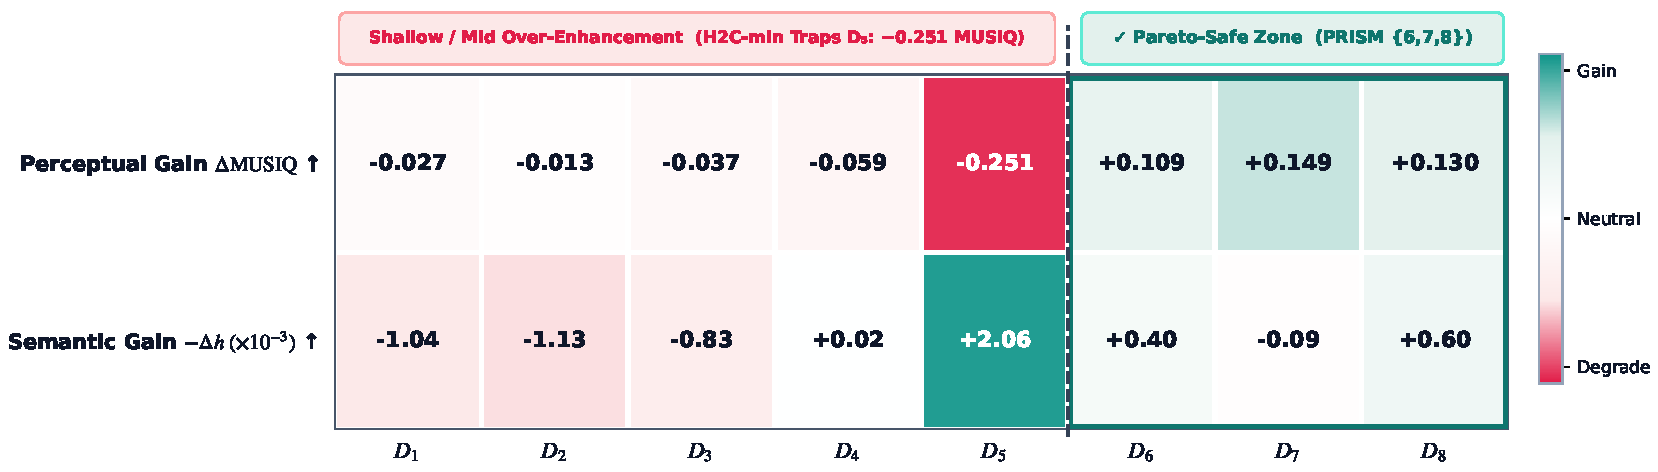
\includegraphics[width=0.92\textwidth]{fig_layer_sensitivity_heatmap.pdf}
\caption{Layer-wise marginal sensitivity heatmap across bottleneck blocks $D_1$--$D_8$ averaged over 3 random seeds (3407/3408/3409). Shallow-to-mid blocks $D_1$--$D_5$ yield negative perceptual gains---peaking at $D_5$ ($-0.251$) despite its high semantic drop---whereas deep blocks $\{D_6,D_7,D_8\}$ unite positive perceptual gains with reliable semantic performance.}
\label{fig:sensitivity}
\end{figure}

\begin{table}[H]\centering\small\setlength{\tabcolsep}{4pt}
\begin{tabular*}{0.94\textwidth}{@{\extracolsep{\fill}}lrrrrrrrr@{}}\toprule
Marginal Metric (3 Seeds) & $D_1$ & $D_2$ & $D_3$ & $D_4$ & $D_5$ & $D_6$ & $D_7$ & $D_8$ \\\midrule
Perceptual Gain $\Delta\mathrm{MUSIQ}\uparrow$ & $-0.027$ & $-0.013$ & $-0.037$ & $-0.059$ & \textcolor{prismred}{$-0.251$} & \best{$+0.109$} & \best{$+0.149$} & \best{$+0.130$} \\
Semantic Gain $-\Delta h\;(\times 10^{-3})\uparrow$ & $-1.04$ & $-1.13$ & $-0.83$ & $+0.02$ & $+2.06$ & $+0.40$ & $-0.09$ & $+0.60$ \\\bottomrule
\end{tabular*}
\caption{Block-wise average marginal inclusion gains across $D_1$--$D_8$ computed over all 168 subset probes (visualized in Figure~\ref{fig:sensitivity}).}
\label{tab:marginal_blocks}
\end{table}

\begin{figure}[H]\centering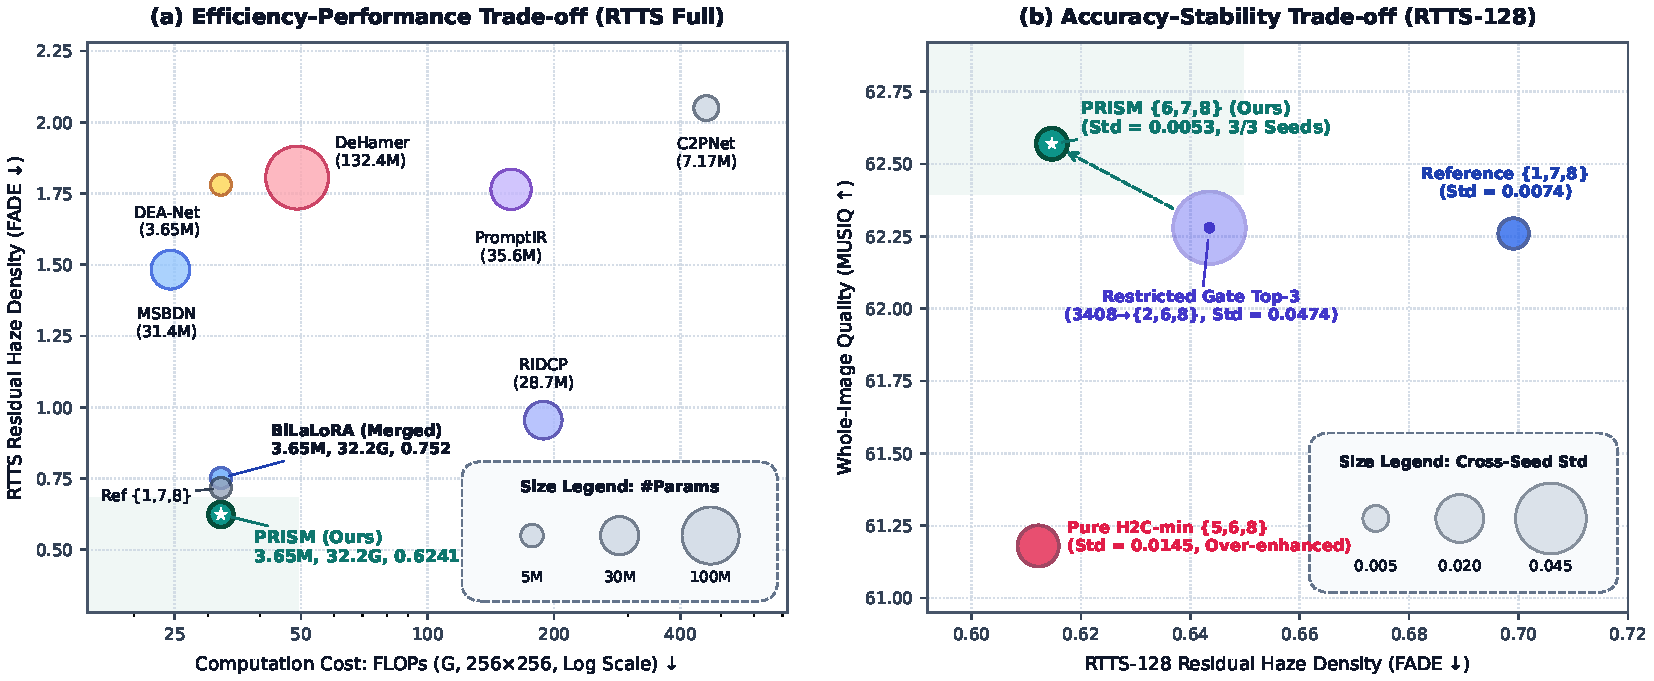
\includegraphics[width=0.92\textwidth]{fig_efficiency_stability_bubble.pdf}
\caption{Three-dimensional efficiency and stability trade-offs. \textbf{(a)} RTTS efficiency--performance plane (256$\times$256 FLOPs vs. FADE, area = parameters): after merging, BiLaLoRA, Ref.~\(\{1,7,8\}\), and \method~all sit at baseline 3.65M params / 32.2G FLOPs, with \method~reaching lowest FADE (0.6241). \textbf{(b)} RTTS-128 quality--stability plane (area = cross-seed FADE std): \method~locks $\{6,7,8\}$ across 3/3 seeds (std 0.0053) while leading MUSIQ (62.57).}
\label{fig:bubble}
\end{figure}

\clearpage
\section{Extended Fattal Qualitative Views \& Boundary Case}
Figure~\ref{fig:fullphotos} provides uncropped full-aspect qualitative comparisons on the Fattal benchmark scenes shown in Figure~\ref{fig:visual} (\texttt{swan}, \texttt{snow}, and \texttt{buildings}, seed 3407). Figure~\ref{fig:traincase} further examines the Fattal \texttt{train\_input.png} boundary case: uncovering dense dark rails and fine gravel lowers perceptual fog density to the lowest in the benchmark (FADE \best{0.1722} vs. Ref.~\(\{1,7,8\}\)+EVA 0.1814 and official BiLaLoRA 0.1953) while trading off mildly against KonIQ-MUSIQ ($58.88 \to 57.92$, unrounded difference $-0.95$) due to exposed high-frequency track textures, echoing the perception--distortion trade-off observed on Dense-Haze.

\begin{figure}[H]\centering\setlength{\tabcolsep}{2pt}\begin{tabular}{cccc}
Hazy Input & BiLaLoRA (Official) & Ref. \{1,7,8\}+EVA & \method \\
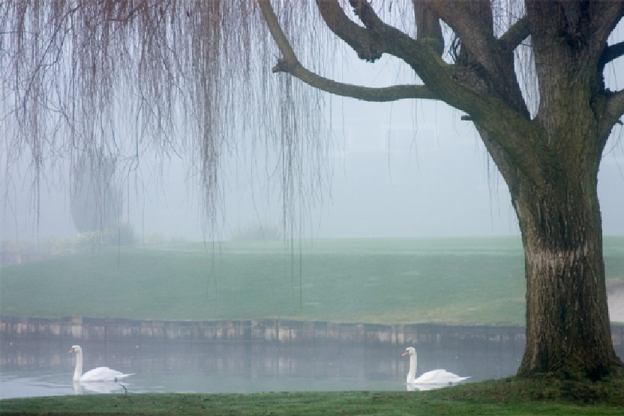
\includegraphics[width=.235\textwidth,height=.18\textwidth,keepaspectratio]{figures/swan_input.png} & 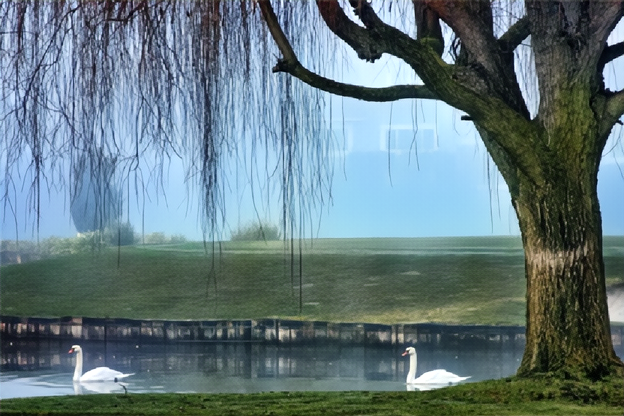
\includegraphics[width=.235\textwidth,height=.18\textwidth,keepaspectratio]{figures/swan_official_bilalora.png} & 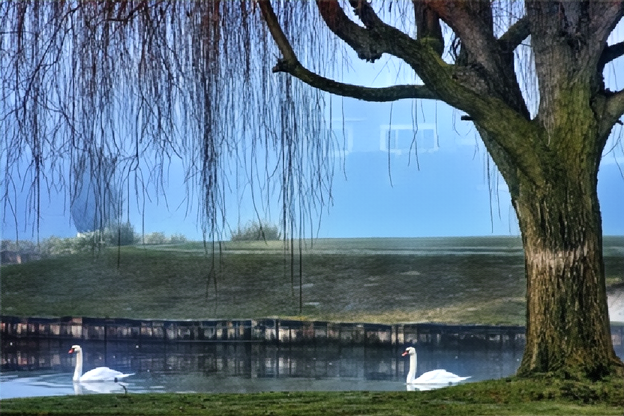
\includegraphics[width=.235\textwidth,height=.18\textwidth,keepaspectratio]{figures/swan_warm_published_3407.png} & 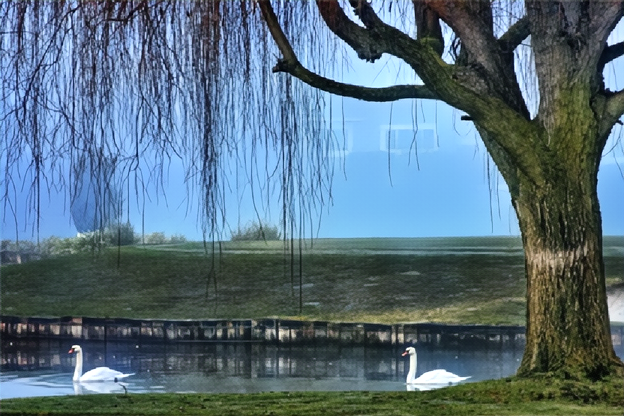
\includegraphics[width=.235\textwidth,height=.18\textwidth,keepaspectratio]{figures/swan_warm_quality_constrained_3407.png} \\[5pt]
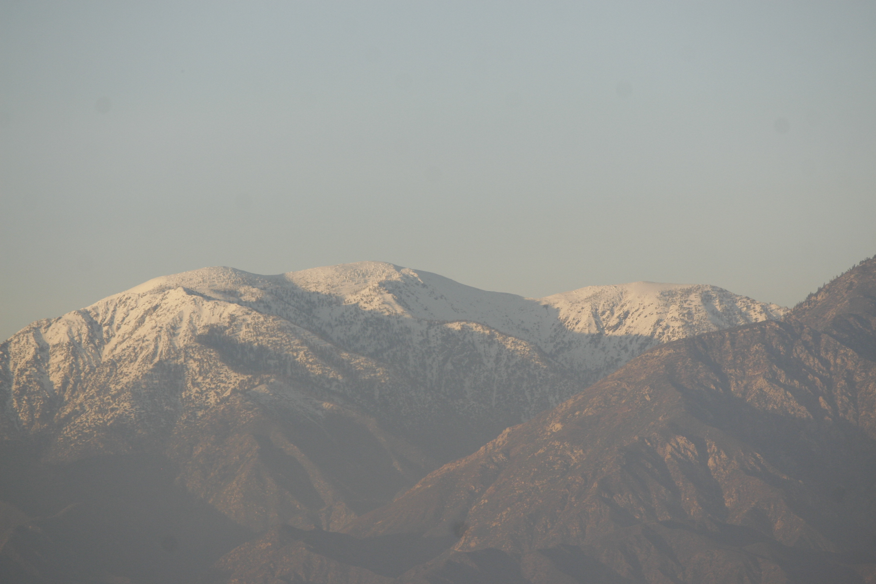
\includegraphics[width=.235\textwidth,height=.18\textwidth,keepaspectratio]{figures/snow_input.png} & 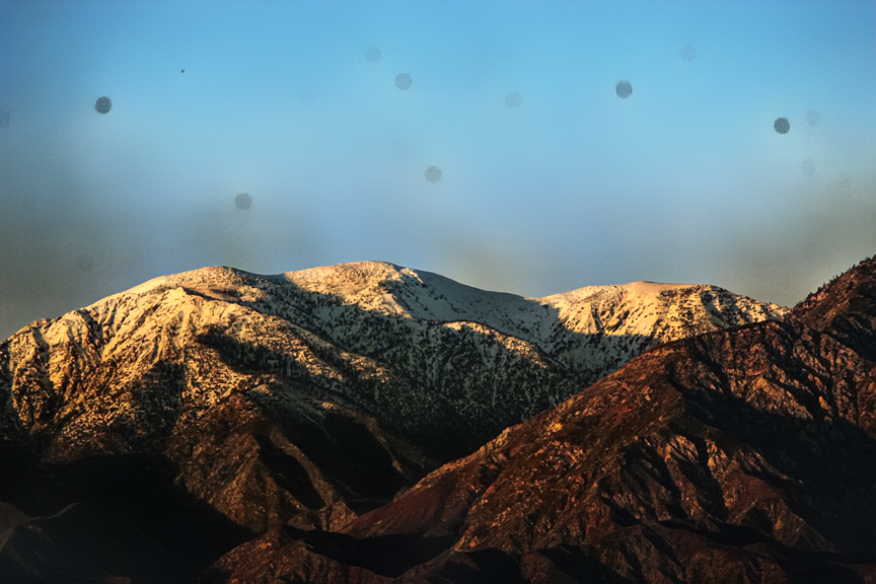
\includegraphics[width=.235\textwidth,height=.18\textwidth,keepaspectratio]{figures/snow_official_bilalora.png} & 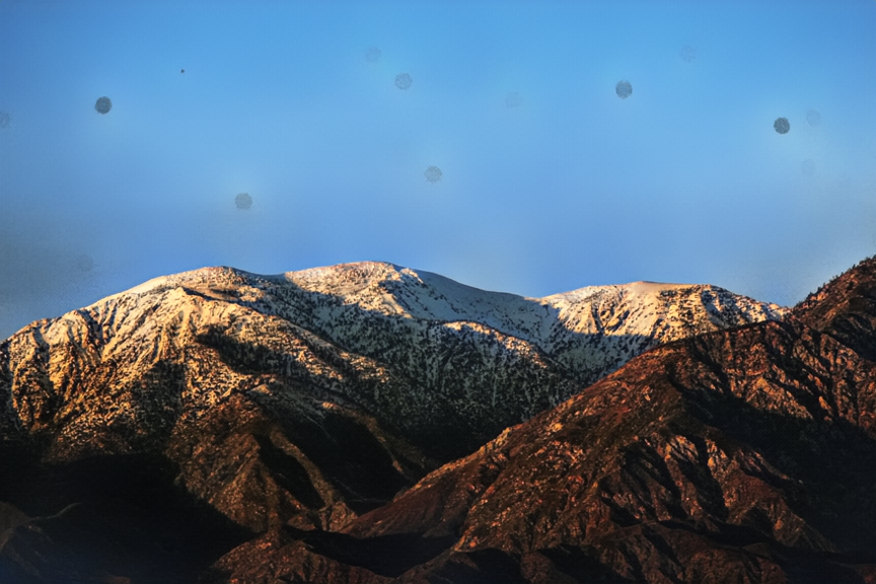
\includegraphics[width=.235\textwidth,height=.18\textwidth,keepaspectratio]{figures/snow_warm_published_3407.png} & 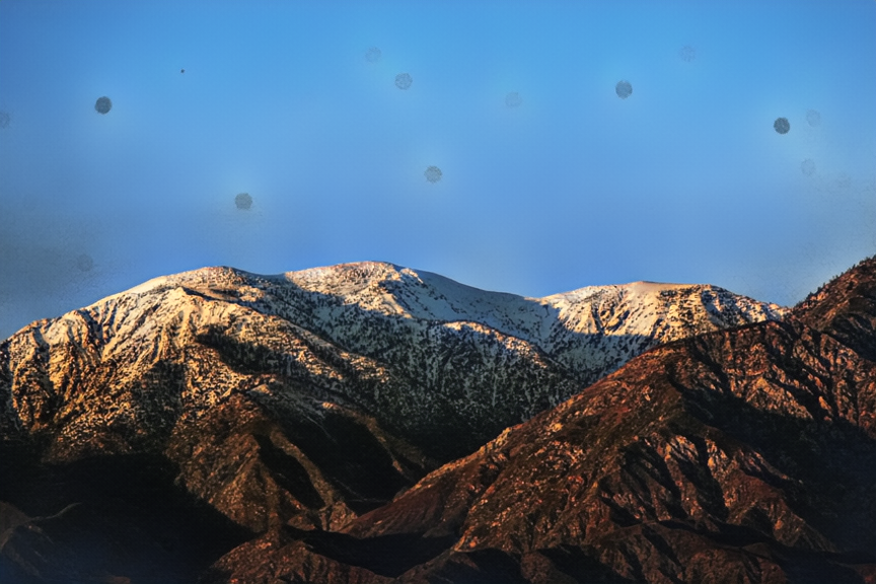
\includegraphics[width=.235\textwidth,height=.18\textwidth,keepaspectratio]{figures/snow_warm_quality_constrained_3407.png} \\[5pt]
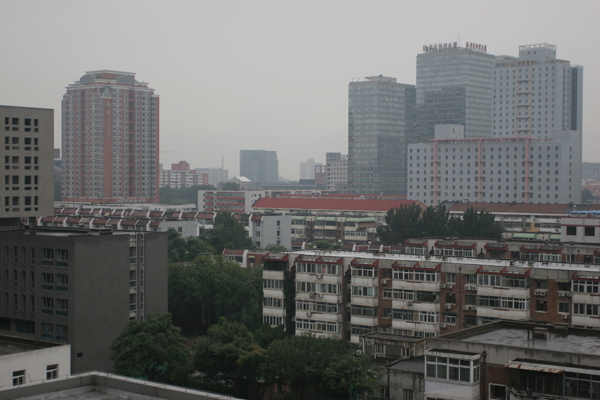
\includegraphics[width=.235\textwidth,height=.18\textwidth,keepaspectratio]{figures/buildings_input.png} & 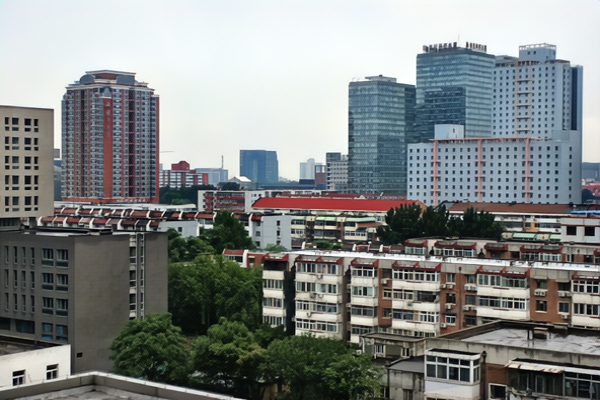
\includegraphics[width=.235\textwidth,height=.18\textwidth,keepaspectratio]{figures/buildings_official_bilalora.png} & 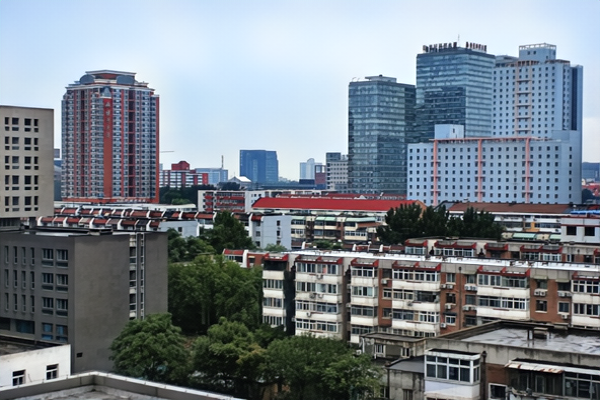
\includegraphics[width=.235\textwidth,height=.18\textwidth,keepaspectratio]{figures/buildings_warm_published_3407.png} & 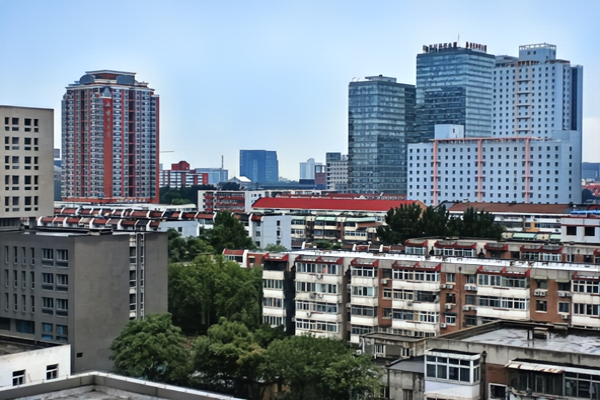
\includegraphics[width=.235\textwidth,height=.18\textwidth,keepaspectratio]{figures/buildings_warm_quality_constrained_3407.png} \\[5pt]
\end{tabular}

\caption{Uncropped full-aspect qualitative views of Figure~\ref{fig:visual} Fattal scenes (\texttt{swan}, \texttt{snow}, \texttt{buildings}).}
\label{fig:fullphotos}
\end{figure}

\begin{figure}[H]\centering\setlength{\tabcolsep}{2pt}\begin{tabular}{ccccc}
Hazy Input & BiLaLoRA (Official) & Ref. \{1,7,8\}+EVA & \method & $8\times$ Diff. \\
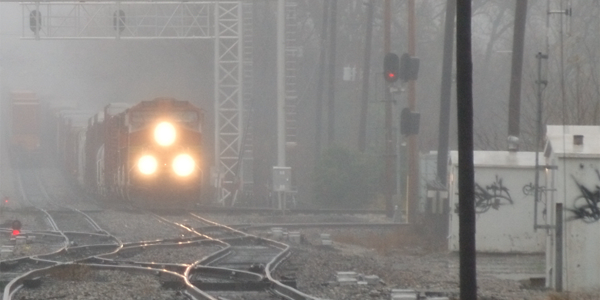
\includegraphics[width=.188\textwidth]{figures/train_input_crop.png} & 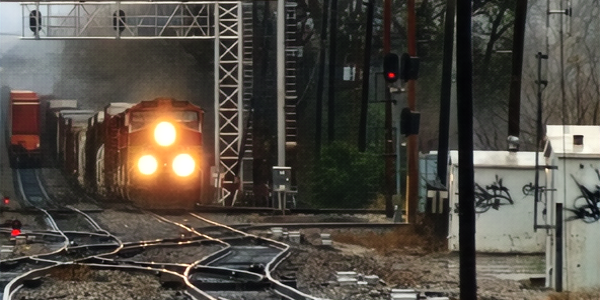
\includegraphics[width=.188\textwidth]{figures/train_official_bilalora_crop.png} & 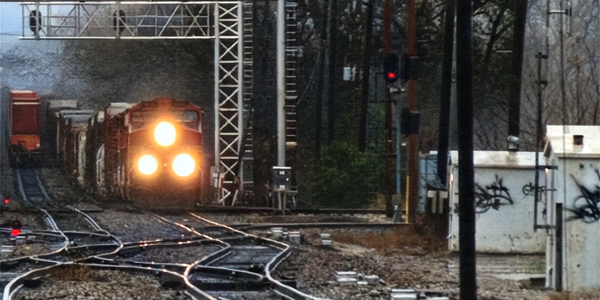
\includegraphics[width=.188\textwidth]{figures/train_warm_published_3407_crop.png} & 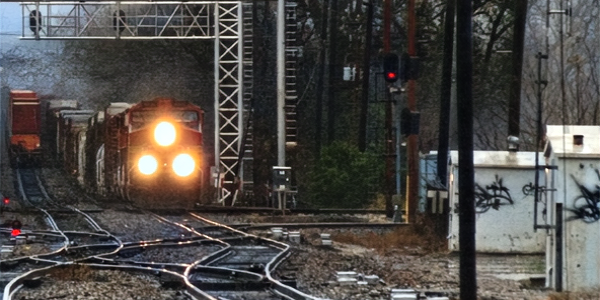
\includegraphics[width=.188\textwidth]{figures/train_warm_quality_constrained_3407_crop.png} & 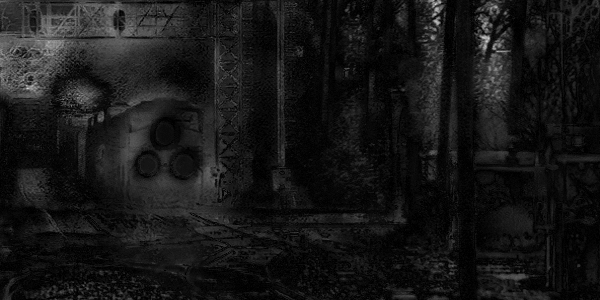
\includegraphics[width=.188\textwidth]{figures/train_difference.png} \\
\footnotesize {\footnotesize \texttt{train}} & {\footnotesize 0.1953 / \best{63.67}} & {\footnotesize 0.1814 / 58.88} & {\footnotesize \best{0.1722} / 57.92} & {\footnotesize $\Delta$MUSIQ=-0.95} \\[5pt]
\end{tabular}

\caption{Fattal boundary case \texttt{train}: $2:1$ zoom comparison and $8\times$ spatial difference (seed 3407).}
\label{fig:traincase}
\end{figure}

\end{document}
